% =============================================================================
% 流体力学（水力学）自学讲义 · 第 1 部分
% 第一章：流体基本性质；第二章：水静力学
% 模式：passive-study · 主题：teal · 图示：TikZ 重绘
% =============================================================================
\documentclass[aspectratio=169,10pt]{beamer}
\usepackage[teal]{template-lib/template-lib}
\uselayout{text}\uselayout{eq}\uselayout{twocol}\uselayout{1img}\uselayout{table}
\usetikzlibrary{arrows.meta,calc,positioning,patterns,decorations.pathmorphing,decorations.pathreplacing,decorations.markings}

% ── 记号缩写 ─────────────────────────────────────────────────────────────────
\newcommand{\rd}{\,\mathrm{d}}
\newcommand{\dd}[2]{\frac{\mathrm{d}#1}{\mathrm{d}#2}}
\newcommand{\pd}[2]{\frac{\partial #1}{\partial #2}}
\newcommand{\DDt}[1]{\frac{\mathrm{D}#1}{\mathrm{D}t}}
\newcommand{\grad}{\nabla}
\newcommand{\divg}{\nabla\!\cdot}
\newcommand{\vc}[1]{\boldsymbol{#1}}
\newcommand{\Real}{\mathbb{R}}
\newcommand{\Rey}{\mathit{Re}}
\newcommand{\atm}{\mathrm{atm}}
\newcommand{\proofskipnote}{\footnote{\scriptsize 非数学背景读者：本帧为\emph{推导细节}，第一遍可先跳过，记住本帧\emph{要点}即可。}}

% 本地化模板中的 takeaway 标签。
\renewcommand{\TLtakeaway}[1]{%
  \vspace{0.25em}%
  \begin{tikzpicture}
    \node[fill=TLaccentLight, rounded corners=3pt, inner sep=7pt,
          text width=\dimexpr\linewidth-14pt\relax, align=justify] {%
      \small\textcolor{TLaccent}{\textbf{要点。}} #1%
    };
  \end{tikzpicture}%
  \vspace{0.1em}%
}

\TLsetfoot{流体力学（水力学）\textperiodcentered{} 自学讲义 \textperiodcentered{} 第 1 部分：基本性质与水静力学}

\begin{document}

% =============================================================================
% A. 标题 + 如何使用
% =============================================================================
\TLtitlecenter
  {流体基本性质与水静力学}
  {流体力学（水力学）自学讲义 \textperiodcentered{} 第 1 部分（第一、二章）}
  {第一章：流体基本性质 \textperiodcentered{} 第二章：水静力学}
  {passive-study 自学讲义}

\begin{frame}{如何使用本讲义}
  这份讲义面向第一次系统学习流体力学的读者：你只需要高等数学、线性代数和基础大学物理，不需要预先学过流体力学。
  \begin{itemize}
    \item 每个概念都会先回答“为什么需要它”，再给定义、公式、图示和可复算的例子。
    \item 非数学或非流体背景读者，请先读下一节“先建直觉”；看到带 \proofskipnote 的推导帧，第一遍可先抓要点，第二遍再补细节。
    \item 关键词会给出英文术语，例如 viscosity、hydrostatic pressure；正文解释均使用中文。
    \item 练习题含由弱到强的 hints；完整 solutions 放在附录，便于你先独立尝试。
  \end{itemize}
  \TLtakeaway{读法：先看图和物理问题，再看公式；每条公式都要问“量纲是什么、方向是什么、基准是什么”。}
\end{frame}

% =============================================================================
% B. 先建直觉
% =============================================================================
\TLsection{先建直觉 · 流体与静水压强在讲什么（新手先读）}

\begin{frame}{流体和固体的差别：剪切一来，谁能静止？}
  \begin{columns}[T]
    \column{0.48\textwidth}
      \begin{itemize}
        \item 固体可以在剪切力下保持静止：桌面受水平推力但未必滑动。
        \item 静止流体不能承受任意小剪切力：只要存在持续剪切，流体就会发生相对运动。
        \item 流体可以承受压力；水桶里的水能被桶壁压住。
        \item 这句话给出本课程的起点：流体的核心特征是\TLterm{易流动性}。
      \end{itemize}
    \column{0.52\textwidth}
      \centering
      \begin{tikzpicture}[scale=0.93,>={Stealth[length=5pt]}]
        \node[draw=TLprimary,fill=TLprimaryTint,minimum width=2.6cm,minimum height=1.35cm,align=center] (solid) at (-1.9,0) {固体\\形状可保持};
        \node[draw=TLaccent,fill=TLaccentLight,minimum width=2.6cm,minimum height=1.35cm,align=center] (fluid) at (1.9,0) {流体\\剪切下流动};
        \draw[->,thick,TLaccent] ($(solid.north west)+(0.15,0.25)$) -- ($(solid.north east)+(0.65,0.25)$) node[midway,above]{剪切力};
        \draw[->,thick,TLaccent] ($(fluid.north west)+(0.15,0.25)$) -- ($(fluid.north east)+(0.65,0.25)$) node[midway,above]{剪切力};
        \draw[TLprimary,thick] (-3.25,-0.9)--(-0.55,-0.9);
        \draw[TLprimary,thick] (-3.25,-1.05)--(-0.55,-1.05);
        \foreach \x in {-3.0,-2.55,-2.1,-1.65,-1.2,-0.75}{\draw[TLinkSoft] (\x,-0.9)--(\x+0.18,-1.05);}
        \draw[TLaccent,thick,decorate,decoration={snake,amplitude=0.5mm,segment length=4mm}] (0.65,-1.0)--(3.25,-1.0);
        \node[TLinkSoft] at (-1.9,-1.45) {可静止};
        \node[TLinkSoft] at (1.9,-1.45) {持续变形};
      \end{tikzpicture}
  \end{columns}
  \TLtakeaway{“流体不能承受剪切力”只在\emph{静止状态}下成立；运动流体会有粘性切应力。}
\end{frame}

\begin{frame}{先认三个物理量：黏度、密度、压强}
  \begin{columns}[T]
    \column{0.56\textwidth}
      \begin{itemize}
        \item \TLterm{黏度}：拖动一块板有多费劲；油比水更“黏”，同样速度梯度下切应力更大。
        \item \TLterm{密度}：同样体积的一桶流体有多重；水约 $1000\,\mathrm{kg/m^3}$，水银约 $13600\,\mathrm{kg/m^3}$。
        \item \TLterm{压强}：单位面积上受到的垂直压力；静水在一点处向各个方向推得一样大。
      \end{itemize}
      \[
        \rho=\frac{m}{V}, \qquad \gamma=\rho g, \qquad p=\frac{F_\perp}{A}.
      \]
    \column{0.44\textwidth}
      \centering
      \begin{tikzpicture}[scale=0.86,>={Stealth[length=4.5pt]}]
        \draw[fill=TLprimaryTint,draw=TLprimary,thick] (-1.25,-1.0) rectangle (1.25,1.0);
        \draw[fill=white,draw=TLprimary,thick] (-1.1,0.55) rectangle (1.1,0.78);
        \draw[->,TLaccent,very thick] (0,1.12)--(0.95,1.12) node[right]{拖板};
        \foreach \y/\len in {-0.75/0.15,-0.45/0.45,-0.15/0.75,0.15/1.05,0.45/1.35}{
          \draw[->,TLprimary] (-0.85,\y)--++(\len,0);
        }
        \node[TLinkSoft] at (0,-1.35) {速度从下到上逐渐增大};
        \draw[->,TLaccent] (1.7,0)--(2.4,0) node[right]{压强};
        \draw[->,TLaccent] (-1.7,0)--(-2.4,0) node[left]{压强};
        \draw[->,TLaccent] (0,1.45)--(0,2.05) node[above]{压强};
      \end{tikzpicture}
  \end{columns}
  \TLtakeaway{黏度回答“剪切时有多抗拒”，密度回答“单位体积有多重”，压强回答“单位面积被推多大”。}
\end{frame}

\begin{frame}{静水压强为什么越深越大？}
  \begin{columns}[T]
    \column{0.48\textwidth}
      \begin{itemize}
        \item 深处的流体要托住上方一摞水柱。
        \item 深度增加 $h$，上方水柱重量增加 $\rho g hA$。
        \item 除以底面积 $A$，压强增加 $\rho g h$。
      \end{itemize}
      \[
        p=p_0+\rho g h.
      \]
      口算：$h=10\,\mathrm{m}$ 的水柱给出
      \[
        \rho g h\approx 1000\times 9.8\times 10
        =9.8\times 10^4\,\mathrm{Pa},
      \]
      约等于一个工程大气压。
    \column{0.52\textwidth}
      \centering
      \begin{tikzpicture}[scale=0.83,>={Stealth[length=5pt]}]
        \fill[TLprimaryTint] (-1.45,-2.0) rectangle (1.45,1.2);
        \draw[TLprimary,thick] (-1.45,1.2)--(1.45,1.2);
        \draw[TLprimary,thick] (-1.45,-2.0)--(-1.45,1.2) (1.45,-2.0)--(1.45,1.2);
        \draw[decorate,decoration={brace,mirror,amplitude=5pt},TLinkSoft] (1.75,1.2)--(1.75,-1.25) node[midway,right=5pt]{$h$};
        \draw[fill=TLaccentLight,draw=TLaccent,thick] (-0.9,-1.25) rectangle (0.9,1.2);
        \node[TLaccent] at (0,-0.05) {上方水柱};
        \draw[->,very thick,TLaccent] (0,-1.25)--(0,-1.85) node[below]{重量 $\rho g hA$};
        \draw[->,thick,TLprimaryDark] (-0.9,-1.25)--(-1.35,-1.25);
        \draw[->,thick,TLprimaryDark] (0.9,-1.25)--(1.35,-1.25);
        \node[TLinkSoft] at (0,1.5) {自由液面压强 $p_0$};
      \end{tikzpicture}
  \end{columns}
  \TLtakeaway{静水基本公式不是背出来的：它就是“上方水柱重量除以面积”。}
\end{frame}

\begin{frame}{质量力与表面力：买菜称重，买房按面积}
  \begin{columns}[T]
    \column{0.55\textwidth}
      \begin{itemize}
        \item \TLterm{质量力}作用在每个流体质点上，按质量或体积累加；重力、惯性力都属于这一类。
        \item 源讲义的比喻：像买菜称重，质量越大，总价越大。
        \item \TLterm{表面力}作用在一个面上，按面积累加；压强和切应力都来自表面力。
        \item 源讲义的比喻：像买房按平米，面积越大，总价越大。
      \end{itemize}
      \[
        \text{质量力总量}=\rho V\,\vc f,\qquad
        \text{表面力总量}=\int_A \vc t\,\rd A.
      \]
    \column{0.45\textwidth}
      \centering
      \begin{tikzpicture}[scale=0.88,>={Stealth[length=5pt]}]
        \draw[fill=TLprimaryTint,draw=TLprimary,thick] (-1.2,-0.9) rectangle (1.2,0.9);
        \foreach \x in {-0.8,-0.4,0,0.4,0.8}{
          \foreach \y in {-0.45,0,0.45}{
            \draw[->,TLaccent] (\x,\y+0.25)--(\x,\y-0.15);
          }
        }
        \node[TLinkSoft] at (0,-1.25) {质量力：每个质点都受力};
        \draw[fill=white,draw=TLprimary,thick] (-1.2,1.7) rectangle (1.2,2.15);
        \foreach \x in {-0.8,-0.35,0.1,0.55,1.0}{
          \draw[->,TLprimaryDark,thick] (\x,2.55)--(\x,2.18);
        }
        \node[TLinkSoft] at (0,2.85) {表面力：作用在接触面上};
      \end{tikzpicture}
  \end{columns}
  \TLtakeaway{后面所有平衡方程，都只是在同一个微团上把“按体积算的力”和“按面积算的力”加起来。}
\end{frame}

\begin{frame}{阅读路径：第一遍抓什么，第二遍补什么}
  \begin{columns}[T]
    \column{0.5\textwidth}
      \TLinfoblock{第一遍必读}{
        \begin{itemize}
          \item 流体定义、连续介质、黏度、密度、压强；
          \item 静水压强公式 $p=p_0+\rho gh$；
          \item 压强测量、总压力、浮力和压力体；
          \item 每个带数字的算例。
        \end{itemize}}
    \column{0.5\textwidth}
      \TLinfoblock{第二遍细读}{
        \begin{itemize}
          \item 静水压强各向同性推导；
          \item 欧拉平衡微分方程推导；
          \item 势函数、无旋条件、等压面；
          \item 压力中心公式的矩推导。
        \end{itemize}}
  \end{columns}
  \medskip
  你需要的背景只有高等数学、线性代数和大学物理；本讲义会在首次使用时解释每个流体力学术语。
  \TLtakeaway{学习路径不是“先背公式”，而是“图像直觉 $\to$ 力平衡 $\to$ 公式 $\to$ 算例”。}
\end{frame}

% =============================================================================
% C. 第一章
% =============================================================================
\TLsection{第一章 · 流体的基本物理性质}

\begin{frame}{流体的定义：为什么剪切力是分界线？}
  \small
  我们需要先回答“研究对象是什么”。流体力学中的流体不是只指水，而是指一类在剪切作用下不能保持静止的连续物质。
  \[
    \boxed{\text{流体：静止时不能承受任意小剪切力，但可以承受压力。}}
  \]
  \begin{itemize}
    \item \TLterm{压力}垂直于受力面；一杯水静止时处处有压力。
    \item \TLterm{剪切力}平行于受力面；如果静止流体内部存在剪切力，就会驱动相邻层发生相对滑动。
    \item 因此水静力学中的静止流体只有压强，没有切应力；流体运动时可因粘性产生切应力。
  \end{itemize}
  \vspace{-0.4em}
  \begin{center}
  \begin{tikzpicture}[scale=0.68,>={Stealth[length=5pt]}]
    \draw[fill=TLprimaryTint,draw=TLprimary,thick] (-2.0,-0.55) rectangle (-0.25,0.55);
    \draw[->,TLaccent,thick] (-1.15,0.95)--(-0.45,0.95) node[right]{剪切};
    \node[TLinkSoft] at (-1.12,-0.9) {流体：会继续变形};
    \draw[fill=TLprimaryTint,draw=TLprimary,thick] (0.55,-0.55) rectangle (2.3,0.55);
    \draw[->,TLprimaryDark,thick] (1.42,1.05)--(1.42,0.6) node[midway,right]{压力};
    \node[TLinkSoft] at (1.42,-0.9) {静水：可承压};
  \end{tikzpicture}
  \end{center}
  \TLtakeaway{“不能承受剪切”不能漏掉“静止时”这三个字；运动流体仍会有粘性切应力。}
\end{frame}

\begin{frame}{连续介质假设：为什么可以用微积分？}
  流体由分子组成，但工程尺度下我们不逐个跟踪分子，而把流体看成连续分布的物质。
  \begin{columns}[T]
    \column{0.54\textwidth}
      \begin{itemize}
        \item \TLterm{连续介质假设}：密度、压强、速度等物理量随空间连续变化，并可求导。
        \item \TLterm{流体微团}：宏观上足够小，所以可视为一点；微观上又足够大，所以含有大量分子。
        \item 在本讲义中，除非特别说明，流体默认满足连续介质假设。
      \end{itemize}
      \[
        \rho(x,y,z),\quad p(x,y,z),\quad \vc u(x,y,z)
      \]
      都被视作空间点上的函数。
    \column{0.46\textwidth}
      \centering
      \begin{tikzpicture}[scale=0.88]
        \draw[fill=TLprimaryTint,draw=TLprimary,thick] (-1.7,-1.15) rectangle (1.7,1.15);
        \foreach \x/\y in {-1.2/0.7,-0.7/0.25,-1.0/-0.5,-0.25/0.75,0.25/0.15,0.8/0.65,1.1/-0.2,0.4/-0.65,-0.45/-0.85}{
          \fill[TLaccent] (\x,\y) circle (1.2pt);
        }
        \draw[TLprimaryDark,very thick] (0,0) circle (0.55);
        \node[TLprimaryDark] at (0,-1.55) {流体微团};
        \draw[->,TLinkSoft,thick] (1.4,1.0) -- (0.5,0.45);
        \node[TLinkSoft,align=center] at (2.25,1.1) {宏观小\\微观大};
      \end{tikzpicture}
  \end{columns}
  \TLtakeaway{连续介质假设把“很多分子”替换成“连续函数”，这正是后面能写 $\partial p/\partial x$ 的原因。}
\end{frame}

\begin{frame}{粘滞性与无滑移：为什么壁面会拖住流体？}
  黏度回答的问题是：相邻流层有相对运动时，流体内部会产生多大的内摩擦力来抵抗剪切变形？
  \begin{columns}[T]
    \column{0.48\textwidth}
      \begin{itemize}
        \item \TLterm{粘滞性}：运动流体内部产生内摩擦力以抵抗剪切变形的性质。
        \item \TLterm{无滑移条件}：贴着固体壁面的流体速度等于壁面速度。
        \item 牛顿平板实验把复杂流动简化为两块平板之间的线性速度剖面。
      \end{itemize}
      若下板静止、上板速度为 $U$、间距为 $h$，则
      \[
        u(y)=\frac{U}{h}\,y,\qquad \dd{u}{y}=\frac{U}{h}.
      \]
    \column{0.52\textwidth}
      \centering
      \begin{center}
      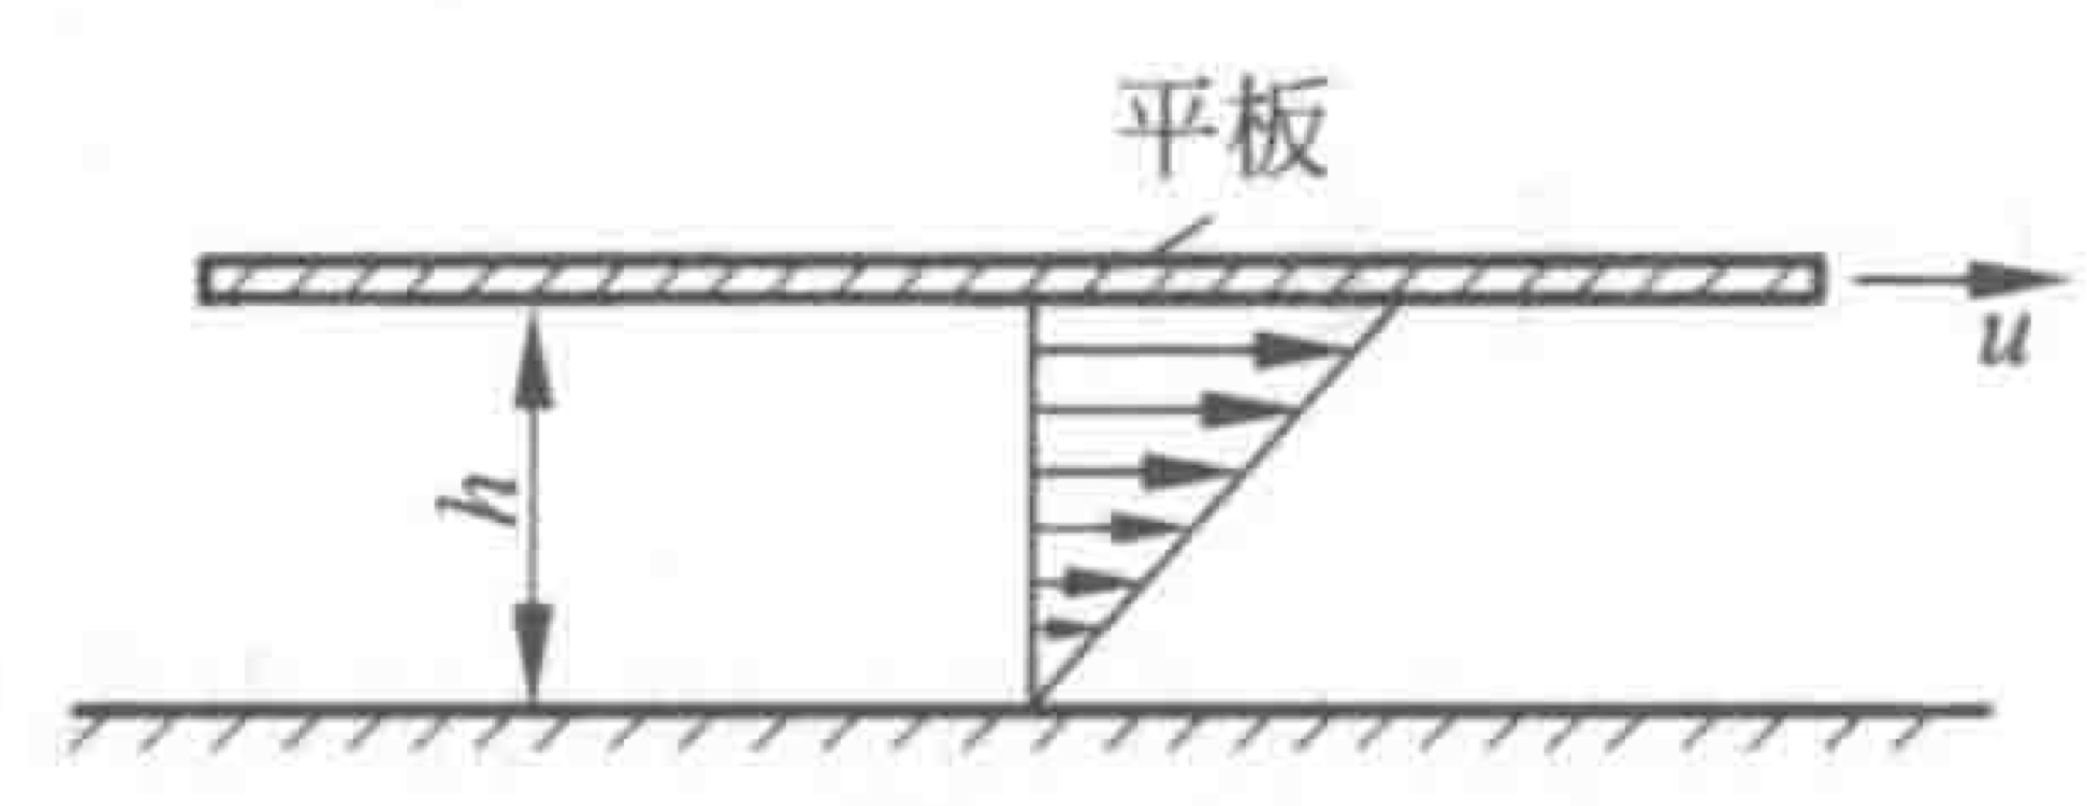
\includegraphics[width=\linewidth,height=0.55\textheight,keepaspectratio]{slides_assets/fluid_deck01/newton-plate.png}\\
      {\scriptsize 图：源讲义原图}
      \end{center}
  \end{columns}
  \TLtakeaway{速度梯度 $\mathrm{d}u/\mathrm{d}y$ 衡量相邻流层滑得有多快；它就是剪切变形速率。}
\end{frame}

\begin{frame}{牛顿内摩擦定律：从总内摩擦力到切应力}
  上一页的平板实验回答一个可测问题：上板匀速运动时，需要多大的外力来抵消流体的内摩擦？
  \[
    F=\mu A\,\dd{u}{y}. \tag{C1}
  \]
  两边除以受力面积 $A$，得到单位面积上的切向内摩擦力：
  \[
    \tau=\frac{F}{A}.
  \]
  \begin{center}
  \begin{tikzpicture}[scale=0.7,>={Stealth[length=5pt]}]
    \draw[fill=TLprimaryTint,draw=TLprimary,thick] (-1.8,-0.55) rectangle (1.8,0.55);
    \draw[fill=white,draw=TLinkSoft,thick] (-2,-0.72) rectangle (2,-0.55);
    \draw[fill=white,draw=TLinkSoft,thick] (-2,0.55) rectangle (2,0.72);
    \draw[->,TLaccent,very thick] (-1.6,0.95)--(-0.4,0.95) node[right]{$F$};
    \node[TLinkSoft] at (0,-1.05) {受力面积 $A$};
  \end{tikzpicture}
  \end{center}
\end{frame}

\begin{frame}{牛顿内摩擦定律：得到局部形式}
  上一帧已经得到总力关系和切应力定义。现在把 $F/A$ 替换为 $\tau$。
  代入式 (C1)：
  \[
    \boxed{\tau=\mu\,\dd{u}{y}}. \tag{C2}
  \]
  \begin{itemize}
    \item $\tau$ 是切应力，单位 $\mathrm{Pa}=\mathrm{N/m^2}$。
    \item $\mu$ 是动力粘度，单位 $\mathrm{Pa\cdot s}$。
    \item $\dd{u}{y}$ 的单位是 $\mathrm{s^{-1}}$，所以右端量纲为 $\mathrm{Pa}$。
  \end{itemize}
  \TLtakeaway{牛顿内摩擦定律只说一件事：牛顿流体中，切应力正比于速度梯度。}
\end{frame}

\begin{frame}{动力粘度与运动粘度：两个“黏”的量不要混}
  \begin{columns}[T]
    \column{0.55\textwidth}
      \begin{itemize}
        \item \TLterm{动力粘度} $\mu$ 直接衡量流体抵抗剪切的能力。
        \item \TLterm{运动粘度} $\nu$ 把动力粘度除以密度，常用于流动相似和雷诺数。
        \item 两者关系为
      \end{itemize}
      \[
        \boxed{\nu=\frac{\mu}{\rho}},\qquad [\nu]=\mathrm{m^2/s}. \tag{C3}
      \]
      \begin{itemize}
        \item 气体升温：分子热运动更剧烈，动量交换增强，$\mu$ 增大。
        \item 液体升温：分子间吸引作用变弱，内摩擦减小，$\mu$ 减小。
      \end{itemize}
    \column{0.45\textwidth}
      \centering
      \begin{tikzpicture}[scale=0.86,>={Stealth[length=5pt]}]
        \draw[->,TLinkSoft] (-0.2,0)--(3.0,0) node[right]{温度 $T$};
        \draw[->,TLinkSoft] (0,-0.15)--(0,2.2) node[above]{$\mu$};
        \draw[TLaccent,very thick] (0.25,0.45).. controls (1.2,0.75) and (2.0,1.25)..(2.75,1.9);
        \draw[TLprimary,very thick] (0.25,1.85).. controls (1.2,1.45) and (2.0,0.9)..(2.75,0.45);
        \node[TLaccent] at (2.15,1.85) {气体};
        \node[TLprimary] at (2.15,0.35) {液体};
      \end{tikzpicture}
  \end{columns}
  \TLtakeaway{$\mu$ 是“力学阻力”，$\nu$ 是“阻力相对于惯性质量的大小”；温度规律对气体和液体相反。}
\end{frame}

\begin{frame}{牛顿流体、非牛顿流体与理想流体}
  牛顿内摩擦定律不是所有流体都满足。分类的依据是 $\tau$ 与剪切变形速率 $\dot\gamma=\mathrm{d}u/\mathrm{d}y$ 的关系。
  \begin{columns}[T]
    \column{0.47\textwidth}
      \begin{itemize}
        \item \TLterm{牛顿流体}：$\tau=\mu\dot\gamma$，图像为过原点直线；水和空气在常见条件下可近似如此。
        \item \TLterm{非牛顿流体}：$\tau$ 与 $\dot\gamma$ 不是线性正比；牙膏、泥浆、血液常需特殊模型。
        \item \TLterm{理想流体}：不考虑粘性，即 $\mu=0$；它不等于“不可压缩流体”。
      \end{itemize}
    \column{0.53\textwidth}
      \centering
      \begin{center}
      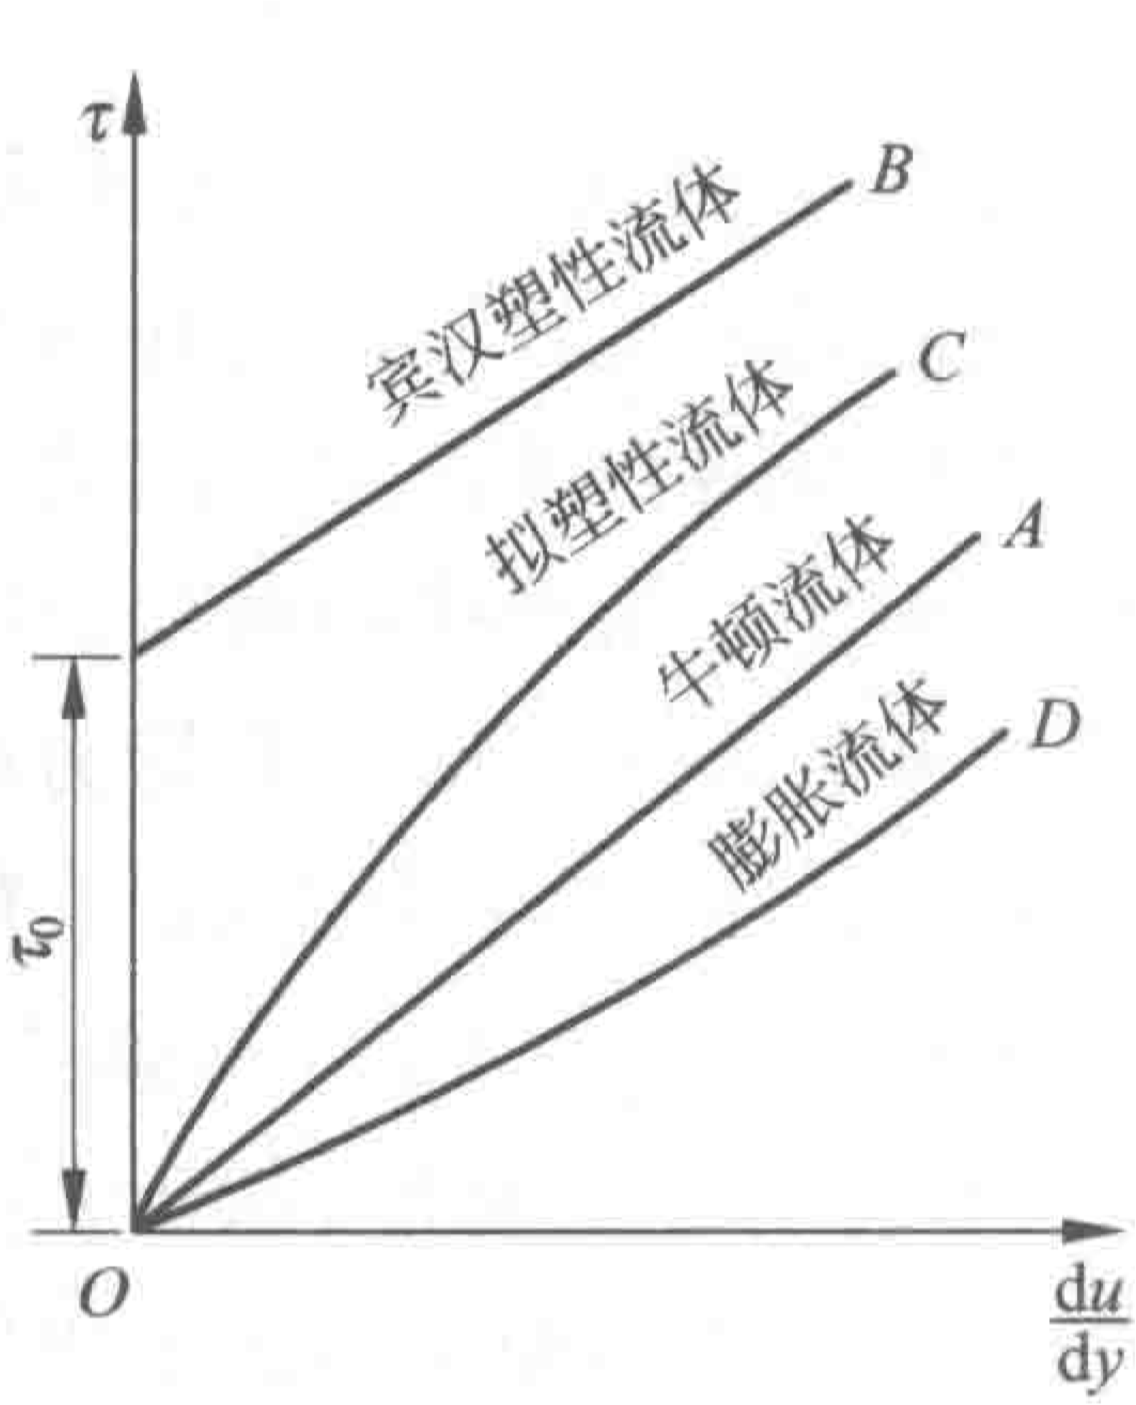
\includegraphics[width=\linewidth,height=0.50\textheight,keepaspectratio]{slides_assets/fluid_deck01/fluid-types.png}\\
      {\scriptsize 图：源讲义原图}
      \end{center}
  \end{columns}
  \TLtakeaway{“理想”只表示无粘；“不可压缩”表示密度近似不变，两者是不同假设。}
\end{frame}

\begin{frame}{密度、重度与相对密度}
  这一组量回答“单位体积中装了多少质量或重量”，是后面静水压强公式的系数。
  \[
    \rho=\frac{m}{V},\qquad
    \gamma=\rho g,\qquad
    s=\frac{\rho}{\rho_{\text{水,标准}}}
      =\frac{\gamma}{\gamma_{\text{水,标准}}}. \tag{C4}
  \]
  \begin{center}
  \begin{tabular}{llll}
    \toprule
    量 & 物理意义 & 常用单位 & 典型数值 \\
    \midrule
    $\rho$ & 单位体积质量 & $\mathrm{kg/m^3}$ & 水约 $1000$ \\
    $\gamma$ & 单位体积重量 & $\mathrm{N/m^3}$ & 水约 $9.8\times10^3$ \\
    $s$ & 相对标准水的密度比 & 无量纲 & 水银约 $13.6$ \\
    \bottomrule
  \end{tabular}
  \end{center}
  标准水通常取 $4^\circ\mathrm{C}$、一个标准大气压下的水，计算中常用 $\rho_{\text{水}}=1000\,\mathrm{kg/m^3}$。
  \TLtakeaway{静水压强斜率是 $\rho g$；密度越大，同样深度给出的压强增量越大。}
\end{frame}

\begin{frame}{压缩性：体积变小为什么要用负号？}
  压缩性回答“多加一点压强，体积会相对缩小多少”。压强增加时 $\rd p>0$，体积变化 $\rd V<0$，所以定义中要加负号使模量为正。
  \[
    \boxed{K=-\frac{\rd p}{\rd V/V}}. \tag{C5}
  \]
  \begin{itemize}
    \item $\rd V/V$ 是体积相对变化量；压缩时它为负。
    \item $K$ 的单位与压强相同，都是 $\mathrm{Pa}$。
    \item $K$ 越大，达到同样体积相对缩小所需的压强增量越大。
  \end{itemize}
  \begin{center}
  \begin{tikzpicture}[scale=0.72,>={Stealth[length=5pt]}]
    \draw[fill=TLprimaryTint,draw=TLprimary,thick] (-2.4,-0.5) rectangle (-0.4,0.5);
    \draw[fill=TLaccentLight,draw=TLaccent,thick] (0.6,-0.35) rectangle (2.1,0.35);
    \draw[->,TLaccent,thick] (-0.2,0)--(0.45,0) node[midway,above]{加压};
    \node at (-1.4,-0.85) {体积 $V$};
    \node at (1.35,-0.85) {体积 $V+\rd V$};
    \node[TLinkSoft] at (1.35,-1.2) {$\rd V<0$};
  \end{tikzpicture}
  \end{center}
  结论：$K$ 越大，流体越难压缩；这是“弹性模量”，不是“压缩容易程度”。
\end{frame}

\begin{frame}{压缩性推导：为什么 $K=\rho\,\mathrm{d}p/\mathrm{d}\rho$？}
  本帧把体积变化改写成密度变化，方便后面判断“密度能否近似不变”。\proofskipnote
  对固定质量 $m=\rho V$ 微分：
  \[
    \rd(\rho V)=0.
  \]
  展开乘积微分：
  \[
    V\,\rd\rho+\rho\,\rd V=0.
  \]
  两边除以 $\rho V$：
  \[
    \frac{\rd\rho}{\rho}=-\frac{\rd V}{V}.
  \]
  代入式 (C5)：
  \[
    \boxed{K=\rho\,\frac{\rd p}{\rd\rho}}. \tag{C6}
  \]
  \TLtakeaway{质量守恒把“体积缩小”翻译为“密度增大”；这就是式 (C6) 的来源。}
\end{frame}

\begin{frame}{体积压缩系数与不可压缩近似}
  体积压缩系数把上一页的关系反过来，直接描述“单位压强增量导致的相对体积缩小”。
  \[
    \boxed{\beta=\frac{1}{K}
      =-\frac{\rd V/V}{\rd p}}. \tag{C7}
  \]
  \begin{itemize}
    \item $K$ 的单位是 $\mathrm{Pa}$；$\beta$ 的单位是 $\mathrm{Pa^{-1}}$。
    \item $K$ 越大，越难压缩；$\beta$ 越大，越容易压缩。
    \item 液体通常可近似不可压缩；水击或水锤问题中，微小压缩性会被压力波放大，不能忽略。
    \item 气体在低速流动中可近似不可压缩；经验界限常取马赫数 $Ma<0.3$。
  \end{itemize}
  \TLtakeaway{把水看成不可压缩是近似，不是定义；近似是否可靠取决于问题尺度与压强变化。}
\end{frame}

\begin{frame}{汽化压强、空化与表面张力}
  有些性质不常进入简单静水计算，却决定工程设备是否会出问题。
  \begin{columns}[T]
    \column{0.55\textwidth}
      \begin{itemize}
        \item \TLterm{汽化压强}：给定温度下液体开始汽化所需达到的饱和蒸气压。
        \item 若局部绝对压强低于汽化压强，液体会形成气泡；气泡在高压区塌陷，可能造成空蚀。
        \item \TLterm{表面张力}：自由表面附近分子受力不平衡，沿表面方向表现出的拉力。
        \item 表面张力系数 $\sigma$ 的单位是 $\mathrm{N/m}$。
      \end{itemize}
    \column{0.45\textwidth}
      \centering
      \begin{tikzpicture}[scale=0.88,>={Stealth[length=4pt]}]
        \fill[TLprimaryTint] (-1.6,-0.85) rectangle (1.6,0.85);
        \draw[TLprimary,thick] (-1.6,0.85)--(1.6,0.85);
        \foreach \x in {-1.2,-0.8,-0.35,0.15,0.65,1.1}{
          \fill[TLprimary] (\x,0.55) circle (1.4pt);
          \draw[->,TLaccent] (\x,0.55)--++(0.28,0);
          \draw[->,TLaccent] (\x,0.55)--++(-0.28,0);
        }
        \draw[fill=white,draw=TLaccent,thick] (0,-0.25) circle (0.38);
        \node[TLaccent] at (0,-0.95) {空化气泡};
        \node[TLinkSoft] at (0,1.18) {表面张力沿自由表面作用};
      \end{tikzpicture}
  \end{columns}
  \TLtakeaway{泵吸水、螺旋桨和高速局部流动常受空化限制；静水公式本身不能替代汽化压强检查。}
\end{frame}

\begin{frame}{算例 C1：先求抛物线速度分布的斜率}
  已知 $\mu=0.05\,\mathrm{Pa\cdot s}$，近壁速度分布为
  \[
    u(y)=1.08-300(0.06-y)^2\quad(\mathrm{m/s}).
  \]
  对 $y$ 求导：
  \[
    \dd{u}{y}= -300\cdot 2(0.06-y)\cdot(-1).
  \]
  整理：
  \[
    \dd{u}{y}=600(0.06-y)=36-600y.
  \]
  本帧只完成一个逻辑动作：从速度函数得到速度梯度。下一帧再把壁面坐标代入。
\end{frame}

\begin{frame}{算例 C1：代入壁面坐标得到切应力}
  壁面 $y=0$ 处：
  \[
    \left.\dd{u}{y}\right|_{y=0}=36\,\mathrm{s^{-1}}.
  \]
  代入牛顿内摩擦定律：
  \[
    \tau_w=\mu\left.\dd{u}{y}\right|_{y=0}
      =0.05\times36=1.8\,\mathrm{Pa}.
  \]
  \TLtakeaway{壁面速度为零不代表壁面速度梯度为零；切应力看的是斜率，不是速度值。}
\end{frame}

\begin{frame}{算例 C2：斜面木块的受力平衡}
  \small
  木块底面积 $A=0.50\times0.50=0.25\,\mathrm{m^2}$，质量 $m=5\,\mathrm{kg}$，油层厚度 $\delta=1\,\mathrm{mm}$，速度 $U=0.25\,\mathrm{m/s}$。斜坡为 $5:12$，所以
  \[
    \sin\theta=\frac{5}{13}.
  \]
  匀速表示沿斜面合力为零；重力沿斜面分量等于粘性阻力：
  \[
    mg\sin\theta=\tau A.
  \]
  油层近似线性速度剖面，故
  \[
    \tau=\mu\frac{U}{\delta}.
  \]
  \vspace{-0.5em}
  \begin{center}
  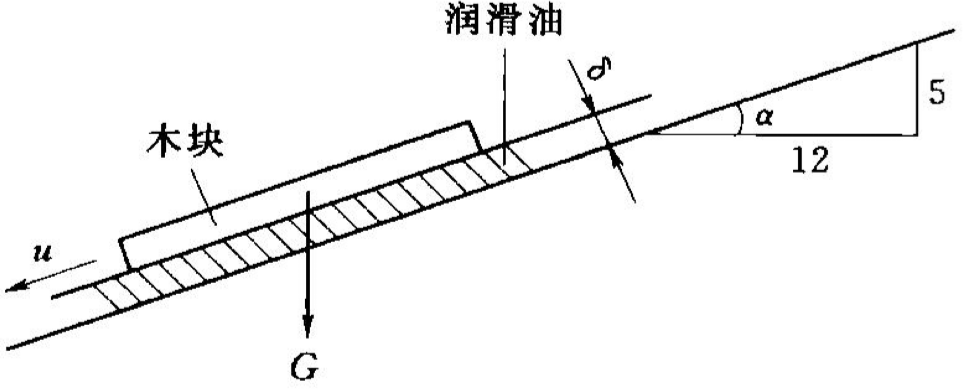
\includegraphics[width=0.7\textwidth,height=0.20\textheight,keepaspectratio]{slides_assets/fluid_deck01/ex-incline-block.png}\\
  {\scriptsize 图：源讲义原图}
  \end{center}
  匀速是本题的关键条件：沿斜面驱动力与粘性阻力相等。
\end{frame}

\begin{frame}{算例 C2：求出动力粘度与运动粘度}
  把 $\tau=\mu U/\delta$ 代入 $mg\sin\theta=\tau A$：
  \[
    mg\sin\theta=\mu\frac{U}{\delta}A.
  \]
  代入并解出动力粘度：
  \[
    \begin{aligned}
    \mu
      &=\frac{mg\sin\theta\,\delta}{AU} \\
      &=\frac{5\times9.8\times(5/13)\times10^{-3}}{0.25\times0.25} \\
      &\approx 0.302\,\mathrm{Pa\cdot s}.
    \end{aligned}
  \]
  油的比重为 $0.92$，$\rho=920\,\mathrm{kg/m^3}$，所以
  \[
    \nu=\frac{\mu}{\rho}\approx \frac{0.302}{920}
       =3.28\times10^{-4}\,\mathrm{m^2/s}.
  \]
\end{frame}

\begin{frame}{算例 C3：圆柱体沿润滑圆管下滑的模型}
  已知数据如下：$d=0.100\,\mathrm{m}$，$L=0.300\,\mathrm{m}$，$G=10\,\mathrm{N}$，$D=0.101\,\mathrm{m}$，$\theta=45^\circ$，$U=0.23\,\mathrm{m/s}$。
  \begin{itemize}
    \item 环形油膜厚度为
      \[
        \delta=\frac{D-d}{2}=0.0005\,\mathrm{m}.
      \]
    \item 圆柱侧面积近似为
      \[
        A=\pi dL=\pi\times0.100\times0.300=9.425\times10^{-2}\,\mathrm{m^2}.
      \]
    \item 匀速下滑表示
      \[
        G\sin\theta=\mu\frac{U}{\delta}A.
      \]
  \end{itemize}
\end{frame}

\begin{frame}{算例 C3：由匀速条件求动力粘度}
  从上一帧的平衡式
  \[
    G\sin\theta=\mu\frac{U}{\delta}A
  \]
  解出 $\mu$：
  \[
    \mu=\frac{G\sin\theta\,\delta}{AU}.
  \]
  解得
  \[
    \begin{aligned}
    \mu
      &=\frac{0.00354}{0.02168} \\
      &\approx0.163\,\mathrm{Pa\cdot s}.
    \end{aligned}
  \]
  \TLtakeaway{共同模板：受力平衡给总粘性力，薄油膜近似给 $\tau=\mu U/\delta$。}
\end{frame}

% =============================================================================
% D. 第二章
% =============================================================================
\TLsection{第二章 · 水静力学}

\begin{frame}{水静力学研究什么：先把“静止”说清楚}
  水静力学要回答两个问题：静止流体内部的压强如何分布，以及这些压强合起来怎样作用在壁面上。
  \begin{columns}[T]
    \column{0.55\textwidth}
      \begin{itemize}
        \item \TLterm{静止}不是说每个分子不动，而是说相邻流体微团之间没有相对位移。
        \item \TLterm{绝对静止}：流体相对惯性参考系静止，只需考虑真实质量力。
        \item \TLterm{相对静止}：流体相对加速参考系静止；在该参考系中还要加入惯性力。
        \item 静止流体不能承受切应力，所以内部受力将从“应力”简化为“压强”。
      \end{itemize}
    \column{0.45\textwidth}
      \centering
      \begin{tikzpicture}[scale=0.82,>={Stealth[length=5pt]}]
        \fill[TLprimaryTint] (-1.7,-1.0) rectangle (1.7,1.0);
        \draw[TLprimary,thick] (-1.7,-1.0) rectangle (1.7,1.0);
        \foreach \x/\lab in {-0.9/A,0/B,0.9/C}{
          \draw[fill=white,draw=TLprimary,thick] (\x,-0.2) circle (0.27);
          \node[TLprimaryDark] at (\x,-0.2) {\lab};
        }
        \draw[<->,TLinkSoft] (-0.63,-0.2)--(-0.27,-0.2);
        \draw[<->,TLinkSoft] (0.27,-0.2)--(0.63,-0.2);
        \node[TLinkSoft,align=center] at (0,-1.45) {相邻微团距离不变\\就是静力学的“静止”};
        \draw[->,TLaccent,very thick] (-1.25,1.35)--(-0.35,1.35) node[right]{参考系可加速};
      \end{tikzpicture}
  \end{columns}
  \TLtakeaway{相对静止并不破坏静力学；它只是把惯性力作为额外质量力放进平衡方程。}
\end{frame}

\begin{frame}{质量力：按质量分配的力}
  我们先把所有力分成两类，因为后面的微元平衡会把这两类力分别相加。
  \begin{itemize}
    \item \TLterm{质量力}又称体积力，作用在流体团中的每个质点上。
    \item 用单位质量流体所受质量力来描述分布：
      \[
        \vc f=f_x\vc i+f_y\vc j+f_z\vc k,\qquad [\vc f]=\mathrm{N/kg}=\mathrm{m/s^2}. \tag{S1}
      \]
    \item 重力沿 $z$ 轴向上为正时写成
      \[
        \vc f=-g\vc k.
      \]
    \item 若参考系有加速度 $\vc a=a_x\vc i+a_y\vc j+a_z\vc k$，相对静止分析中加入惯性力
      \[
        \vc f_{\mathrm{in}}=-a_x\vc i-a_y\vc j-a_z\vc k.
      \]
  \end{itemize}
  \TLtakeaway{质量力的符号由坐标轴决定；本章默认 $z$ 轴向上，所以重力分量是 $f_z=-g$。}
\end{frame}

\begin{frame}{表面力：按面积分配的力}
  表面力回答“相邻流体或壁面通过接触面对这团流体怎样推或拖”。它可以作用在真实边界，也可以作用在流体内部任意假想切面上。
  \begin{columns}[T]
    \column{0.54\textwidth}
      \begin{itemize}
        \item \TLterm{应力}是单位面积上的表面力。
        \item 应力分成垂直于面的\TLterm{正应力} $\sigma$ 和平行于面的\TLterm{切应力} $\tau$。
        \item 静止流体没有切应力，某点的\TLterm{静水压强} $p$ 等于该处压应力的大小。
        \item 压强的单位是 $\mathrm{Pa}=\mathrm{N/m^2}$。
      \end{itemize}
    \column{0.46\textwidth}
      \centering
      \begin{tikzpicture}[scale=0.86,>={Stealth[length=5pt]}]
        \draw[fill=TLprimaryTint,draw=TLprimary,thick] (-1.35,-0.85) rectangle (1.35,0.85);
        \draw[TLprimaryDark,thick] (0,-1.05)--(0,1.05);
        \draw[->,TLaccent,thick] (0.78,0.15)--(0.12,0.15) node[midway,above]{$\sigma$};
        \draw[->,TLaccent,thick] (0.1,-0.55)--(0.1,0.2) node[midway,left]{$\tau$};
        \node[TLinkSoft,align=center] at (0,-1.45) {静止流体：$\tau=0$，只留下压强 $p$};
      \end{tikzpicture}
  \end{columns}
  \TLtakeaway{后面说“压强作用在某个面上”，意思是这个面受到垂直于面的压应力。}
\end{frame}

\begin{frame}{静水压强两特性：要证明哪两件事？}
  压强若要成为一个点函数 $p(x,y,z)$，必须先排除两个疑问：方向会不会不同，作用方向会不会斜着拖动。
  \begin{enumerate}
    \item \textbf{垂直性}：静水压强在作用面上产生的力垂直指向作用面，并且是压力。
    \item \textbf{各向同性}：静止流体中同一点处，任意方向作用面上的压强大小相同。
  \end{enumerate}
  \begin{center}
  \begin{tikzpicture}[scale=0.75,>={Stealth[length=5pt]}]
    \fill[TLprimaryTint] (-2.0,-0.7) rectangle (2.0,0.9);
    \draw[TLprimary,thick] (-2.0,-0.7) rectangle (2.0,0.9);
    \draw[TLprimaryDark,thick] (-0.9,-0.7)--(0.9,0.9);
    \draw[->,TLaccent,thick] (0.2,0.28)--(-0.38,0.93) node[above]{$p_n$};
    \draw[->,TLaccent,thick] (-1.0,0.1)--(-1.55,0.1) node[left]{$p$};
    \draw[->,TLaccent,thick] (1.0,0.1)--(1.55,0.1) node[right]{$p$};
    \node[TLinkSoft] at (0,-1.15) {同一点，换不同方向的小面，压强大小仍相同};
  \end{tikzpicture}
  \end{center}
  \TLtakeaway{垂直性来自“静止无剪切”；各向同性来自“极小微元的表面力平衡”。}
\end{frame}

\begin{frame}{特性一：为什么压强力必须垂直于作用面？}
  本帧只证明方向，不证明大小是否与方向有关。设某静止流体内部取一小面，表面力可分解为法向分量和切向分量。
  \[
    \vc t=\underbrace{\vc t_n}_{\text{垂直于面}}+
          \underbrace{\vc t_\tau}_{\text{平行于面}}.
  \]
  若 $\vc t_\tau\ne\vc 0$，这个切向表面力会使小面两侧流体层发生相对滑动；这与“静止流体微团间无相对位移”矛盾。
  因此
  \[
    \vc t_\tau=\vc 0,\qquad \vc t=\vc t_n.
  \]
  流体内部只能互相压推，不能互相拉开，所以静水压强对应的是指向作用面的压力。
  \TLtakeaway{压强力不沿面“擦过去”；它沿面的法线方向“压过去”。}
\end{frame}

\begin{frame}{特性二的微元：用四面体比较四个方向}
  现在证明同一点处不同方向的压强相同。取一个极小四面体，三个面垂直于坐标轴，斜面面积为 $\rd A$。\proofskipnote
  \begin{columns}[T]
    \column{0.48\textwidth}
      \begin{itemize}
        \item 斜面外法线为 $\vc n=(n_x,n_y,n_z)$。
        \item 斜面在三个坐标面上的投影面积为
          \[
            \begin{aligned}
              \rd A_x&=n_x\rd A,\\
              \rd A_y&=n_y\rd A,\\
              \rd A_z&=n_z\rd A.
            \end{aligned} \tag{S2}
          \]
        \item 质量力与体积成正比，是 $O(\ell^3)$；表面压力与面积成正比，是 $O(\ell^2)$。
      \end{itemize}
    \column{0.52\textwidth}
      \centering
      \begin{tikzpicture}[scale=0.9,>={Stealth[length=5pt]}]
        \coordinate (O) at (0,0);
        \coordinate (X) at (2.4,0);
        \coordinate (Y) at (0,1.55);
        \coordinate (Z) at (-0.75,-0.85);
        \fill[TLprimaryTint] (X)--(Y)--(Z)--cycle;
        \draw[TLprimary,thick] (O)--(X) (O)--(Y) (O)--(Z);
        \draw[TLprimaryDark,thick] (X)--(Y)--(Z)--cycle;
        \draw[->,TLaccent,thick] (0.7,0.55)--(1.15,1.0) node[right]{$p_n\rd A$};
        \draw[->,TLprimaryDark,thick] (-0.35,0.12)--(-1.0,0.12) node[left]{$p_x\rd A_x$};
        \draw[->,TLprimaryDark,thick] (0.55,-0.3)--(0.55,-0.95) node[below]{$p_z\rd A_z$};
        \node[TLinkSoft] at (1.25,-1.15) {斜面投影决定各方向面积};
      \end{tikzpicture}
  \end{columns}
  \TLtakeaway{推导的核心尺度判断：缩小微元时，体力比面力低一阶，极限中不会决定方向压强。}
\end{frame}

\begin{frame}{特性二的推导：先取 $x$ 方向平衡}
  上一帧建立了投影面积关系。本帧只取 $x$ 方向平衡，目标是得到 $p_x=p_n$。\proofskipnote
  \[
    p_x\,\rd A_x-p_n n_x\,\rd A+O(\ell^3)=0.
  \]
  代入 $\rd A_x=n_x\rd A$：
  \[
    (p_x-p_n)n_x\,\rd A+O(\ell^3)=0.
  \]
  两边除以 $\rd A=O(\ell^2)$：
  \[
    (p_x-p_n)n_x+O(\ell)=0.
  \]
  让微元尺寸 $\ell\to0$，若斜面不是与 $x$ 轴正交的退化情形，$n_x\ne0$，于是
  \[
    p_x=p_n.
  \]
  \TLtakeaway{$x$ 方向只用了两件事：投影面积 $\rd A_x=n_x\rd A$，以及体力在极限中比面力低一阶。}
\end{frame}

\begin{frame}{特性二的推导：完成三个方向并得到标量压强}
  上一帧得到 $p_x=p_n$。现在对 $y,z$ 方向重复同样的平衡步骤；这里不省略代数形式。\proofskipnote
  \[
    p_y\,\rd A_y-p_n n_y\,\rd A+O(\ell^3)=0
    \quad\Longrightarrow\quad
    (p_y-p_n)n_y+O(\ell)=0.
  \]
  令 $\ell\to0$，得到
  \[
    p_y=p_n.
  \]
  对 $z$ 方向：
  \[
    p_z\,\rd A_z-p_n n_z\,\rd A+O(\ell^3)=0
    \quad\Longrightarrow\quad
    p_z=p_n.
  \]
  因此同一点处 $p_x=p_y=p_z=p_n$。
  \TLtakeaway{压强可以写成标量 $p(x,y,z)$，因为同一点处它不依赖小面的空间方向。}
\end{frame}

\begin{frame}{欧拉平衡方程：微元六面体要回答什么？}
  静水压强已经是标量。下一步要问：若流体中有质量力，压强在空间中必须怎样变化才能让每个微元平衡？
  \begin{columns}[T]
    \column{0.52\textwidth}
      \begin{itemize}
        \item 取边长为 $\Delta x,\Delta y,\Delta z$ 的小六面体。
        \item 六个面上只有法向压强力。
        \item 体内每一点还受单位质量力 $\vc f=(f_x,f_y,f_z)$。
        \item 微元体积为 $\Delta V=\Delta x\Delta y\Delta z$。
      \end{itemize}
    \column{0.48\textwidth}
      \centering
      \begin{tikzpicture}[scale=0.86,>={Stealth[length=5pt]}]
        \draw[fill=TLprimaryTint,draw=TLprimary,thick] (-1.4,-0.75) rectangle (1.4,0.75);
        \draw[->,TLaccent,thick] (-2.05,0)--(-1.43,0) node[midway,above]{$p_L$};
        \draw[->,TLaccent,thick] (2.05,0)--(1.43,0) node[midway,above]{$p_R$};
        \draw[->,TLprimaryDark,thick] (0,0)--(0.95,-0.45) node[right]{$\rho\vc f\,\Delta V$};
        \draw[<->,TLinkSoft] (-1.4,-1.0)--(1.4,-1.0) node[midway,below]{$\Delta x$};
        \draw[<->,TLinkSoft] (1.65,-0.75)--(1.65,0.75) node[midway,right]{$\Delta z$};
        \node[TLinkSoft] at (0,1.15) {这里只画 $x$-$z$ 截面};
      \end{tikzpicture}
  \end{columns}
  \TLtakeaway{欧拉平衡方程就是“六面压强力 + 质量力 = 0”在微元极限下的结果。}
\end{frame}

\begin{frame}{欧拉平衡方程：先写 $x$ 方向两侧压力}
  本帧只做 $x$ 方向。令微元中心处压强为 $p$，在左右两个面用一阶近似表示压强。\proofskipnote
  \[
    p_L=p-\pd{p}{x}\frac{\Delta x}{2},\qquad
    p_R=p+\pd{p}{x}\frac{\Delta x}{2}.
  \]
  左面压力沿 $+x$ 方向，右面压力沿 $-x$ 方向。两面面积均为 $\Delta y\Delta z$，所以表面力合量为
  \[
    F_{p,x}=p_L\Delta y\Delta z-p_R\Delta y\Delta z.
  \]
  代入 $p_L,p_R$：
  \[
    F_{p,x}
      =-\pd{p}{x}\Delta x\Delta y\Delta z
      =-\pd{p}{x}\Delta V.
  \]
  质量力在 $x$ 方向为
  \[
    F_{f,x}=\rho f_x\Delta V.
  \]
\end{frame}

\begin{frame}{欧拉平衡方程：由平衡得到 $x$ 分量}
  上一帧得到 $x$ 方向两类力：表面压强力 $-\partial p/\partial x\,\Delta V$，质量力 $\rho f_x\Delta V$。\proofskipnote
  平衡条件是二者相加为零：
  \[
    -\pd{p}{x}\Delta V+\rho f_x\Delta V=0.
  \]
  因为微元体积 $\Delta V>0$，两边除以 $\Delta V$：
  \[
    \pd{p}{x}=\rho f_x.
  \]
\end{frame}

\begin{frame}{欧拉平衡方程：三个分量与物理意义}
  $y,z$ 方向也逐面写压力差；得到的分量式为
  \[
    \pd{p}{y}=\rho f_y,\qquad
    \pd{p}{z}=\rho f_z.
  \]
  合写为
  \[
    \boxed{\pd{p}{x_i}=\rho f_i\qquad(i=1,2,3).} \tag{S3}
  \]
  \TLtakeaway{质量力方向就是压强增长方向；若 $f_z=-g$，压强随 $z$ 向上增大而减小。}
\end{frame}

\begin{frame}{压强差公式：把偏导数组装成一个微分}
  欧拉平衡方程给出三个方向上的压强增长率。若从点 $(x,y,z)$ 移动一个小位移
  \[
    \rd\vc r=(\rd x,\rd y,\rd z),
  \]
  压强的一阶增量为
  \[
    \rd p=\pd{p}{x}\rd x+\pd{p}{y}\rd y+\pd{p}{z}\rd z.
  \]
  把式 (S3) 代入：
  \[
    \boxed{\rd p=\rho(f_x\rd x+f_y\rd y+f_z\rd z)
      =\rho\,\vc f\cdot\rd\vc r.} \tag{S4}
  \]
  \vspace{-0.4em}
  \begin{center}
  \begin{tikzpicture}[scale=0.68,>={Stealth[length=5pt]}]
    \draw[->,TLinkSoft] (-2.1,0)--(2.3,0) node[right]{$x$};
    \draw[->,TLinkSoft] (0,-0.95)--(0,1.45) node[above]{$z$};
    \draw[->,TLprimary,very thick] (-0.6,-0.25)--(1.0,0.75) node[right]{$\rd\vc r$};
    \draw[->,TLaccent,very thick] (-0.6,-0.25)--(-0.05,-0.85) node[below]{$\vc f$};
    \node[TLinkSoft] at (0,-1.2) {$\vc f$ 在位移方向上的投影决定 $\rd p$};
  \end{tikzpicture}
  \end{center}
\end{frame}

\begin{frame}{质量力势函数：什么时候能把力写成一个势？}
  对均质不可压缩流体，$\rho$ 为常数。式 (S4) 可写成
  \[
    \rd\!\left(\frac{p}{\rho}\right)
      =f_x\rd x+f_y\rd y+f_z\rd z.
  \]
  左端是全微分，因此右端也必须是某个函数的全微分。设这个函数为 $W$，则必须有
  \[
    \begin{aligned}
      \pd{f_x}{y}-\pd{f_y}{x}&=0,\\
      \pd{f_y}{z}-\pd{f_z}{y}&=0,\\
      \pd{f_z}{x}-\pd{f_x}{z}&=0.
    \end{aligned} \tag{S5}
  \]
  这三式就是 $\nabla\times\vc f=\vc0$ 的分量写法，表示质量力无旋，也叫有势或保守。
  \TLtakeaway{势函数不是新的力；它是把无旋质量力压缩成一个标量函数 $W$ 的记账方式。}
\end{frame}

\begin{frame}{质量力势函数：积分得到静压传递}
  若存在质量力势 $W$，则
  \[
    \vc f=\grad W,\qquad
    f_x\rd x+f_y\rd y+f_z\rd z=\rd W.
  \]
  代回压强差公式：
  \[
    \rd p=\rho\,\rd W.
  \]
  对均质不可压缩流体，沿任意路径从参考点 $0$ 积分到当前点：
  \[
    \int_{p_0}^{p}\rd p=\rho\int_{W_0}^{W}\rd W.
  \]
  因此
  \[
    \boxed{p=p_0+\rho(W-W_0).} \tag{S6}
  \]
  若边界压强 $p_0$ 增加同一个常数，右端所有点的 $p$ 也增加同一个常数，这就是帕斯卡定律或静压传递原理。
  \TLtakeaway{静止液体会等值传递外加压强；压强的空间差异来自势函数差 $W-W_0$。}
\end{frame}

\begin{frame}{等压面：压强不变的面必须怎样放？}
  \TLterm{等压面}是压强相同的点组成的面。沿这个面移动时 $\rd p=0$，代入式 (S4)：
  \[
    \boxed{\vc f\cdot\rd\vc r=0.} \tag{S7}
  \]
  这给出两个性质：
  \begin{itemize}
    \item 等压面上任意切向位移 $\rd\vc r$ 都与质量力 $\vc f$ 正交。
    \item 对均质不可压缩静止流体，等压面也是等势面，因为 $\rd p=\rho\,\rd W$。
  \end{itemize}
  \begin{center}
  \begin{tikzpicture}[scale=0.76,>={Stealth[length=5pt]}]
    \draw[TLprimary,thick] (-2.4,0.55).. controls (-1.1,0.9) and (0.7,0.2)..(2.4,0.55);
    \draw[TLprimary,thick] (-2.4,-0.25).. controls (-1.1,0.1) and (0.7,-0.6)..(2.4,-0.25);
    \draw[->,TLaccent,very thick] (0,0.15)--(0,-1.1) node[below]{$\vc f$};
    \draw[->,TLprimaryDark,thick] (-0.8,0.35)--(0.25,0.18) node[right]{$\rd\vc r$};
    \node[TLinkSoft] at (0,1.05) {等压面切线方向};
  \end{tikzpicture}
  \end{center}
  \TLtakeaway{自由液面和两种静止液体的交界面都是常见等压面；它们必须与有效质量力正交。}
\end{frame}

\begin{frame}{只有重力：从 $\rd p$ 推到静水基本公式}
  最常见情形是只有重力。取 $z$ 轴向上，则 $\vc f=-g\vc k$，所以式 (S4) 变成\proofskipnote
  \[
    \rd p=\rho(0\rd x+0\rd y-g\rd z)=-\rho g\,\rd z.
  \]
  对均质不可压缩液体，$\rho$ 为常数，移项后得到
  \[
    \rd\!\left(z+\frac{p}{\rho g}\right)=0.
  \]
  因此
  \[
    \boxed{z+\frac{p}{\rho g}=C.} \tag{S8}
  \]
  若自由液面处 $z=z_0$、$p=p_0$，当前点深度定义为 $h=z_0-z$，则
  \[
    \boxed{p=p_0+\rho g(z_0-z)=p_0+\rho g h.} \tag{S9}
  \]
  \TLtakeaway{$h$ 是从自由液面向下量的深度；深度向下为正时，压强按 $\rho gh$ 线性增加。}
\end{frame}

\begin{frame}{压强的三种表示：数值、几个大气压、液柱高}
  静水公式给出的是压强，工程上常把同一个压强换成三种等价语言。
  \begin{center}
  \small
  \begin{tabular}{lll}
    \toprule
    表示方式 & 写法 & 典型换算 \\
    \midrule
    SI 压强 & $\mathrm{Pa},\mathrm{kPa},\mathrm{MPa}$ & $1\,\mathrm{Pa}=1\,\mathrm{N/m^2}$ \\
    标准大气压 & $\atm$ & $1\,\atm=1.013\times10^5\,\mathrm{Pa}$ \\
    标准大气压液柱 & 水银柱或水柱 & $76\,\mathrm{cmHg}=10.33\,\mathrm{mH_2O}$ \\
    工程大气压 & $\mathrm{at}$ & $0.981\times10^5\,\mathrm{Pa}=10\,\mathrm{mH_2O}$ \\
    \bottomrule
  \end{tabular}
  \end{center}
  用液柱高表示时，本质上是把 $p=\rho gh$ 反解为
  \[
    h=\frac{p}{\rho g}.
  \]
  \TLtakeaway{液柱高不是另一种物理量；它只是把压强除以该液体的 $\rho g$。}
\end{frame}

\begin{frame}{绝对压强、表压强与真空压强}
  压强数值必须说明基准。水力学中若无特殊说明，常说的压强多指相对当地大气压的表压强。
  \begin{columns}[T]
    \column{0.54\textwidth}
      \begin{itemize}
        \item \TLterm{绝对压强} $p_{\mathrm{abs}}$：以绝对真空为零点。
        \item \TLterm{相对压强}或表压强：
          \[
            p_g=p_{\mathrm{abs}}-p_a.
          \]
        \item 若 $p_{\mathrm{abs}}<p_a$，定义\TLterm{真空压强}：
          \[
            p_v=p_a-p_{\mathrm{abs}}=-p_g.
          \]
        \item 真空度最大为当地大气压 $p_a$，因为绝对压强不能小于零。
      \end{itemize}
    \column{0.46\textwidth}
      \centering
      \begin{tikzpicture}[scale=0.82,>={Stealth[length=5pt]}]
        \draw[->,TLinkSoft,thick] (0,0)--(0,3.2) node[above]{压强};
        \draw[TLprimary,thick] (-1.2,0)--(1.2,0) node[right]{绝对真空};
        \draw[TLaccent,thick] (-1.2,1.55)--(1.2,1.55) node[right]{$p_a$};
        \draw[TLprimaryDark,thick] (-1.2,2.55)--(1.2,2.55) node[right]{$p_{\mathrm{abs}}>p_a$};
        \draw[TLprimaryDark,thick] (-1.2,0.75)--(1.2,0.75) node[right]{$p_{\mathrm{abs}}<p_a$};
        \draw[<->,TLprimary] (-0.75,1.55)--(-0.75,2.55) node[midway,left]{$p_g$};
        \draw[<->,TLaccent] (0.75,0.75)--(0.75,1.55) node[midway,right]{$p_v$};
      \end{tikzpicture}
  \end{columns}
  \TLtakeaway{表压可正可负；真空压强只在低于当地大气压时使用，且最大值是 $p_a$。}
\end{frame}

\begin{frame}{水头：把单位重量液体的能量写成长度}
  对只有重力的静止液体，式 (S8) 说明 $z+p/(\rho g)$ 为常数。这里每一项都具有长度单位。
  \begin{itemize}
    \item \TLterm{位置水头} $z$：单位重量液体具有的重力势能。
    \item \TLterm{压强水头} $p/(\rho g)$：单位重量液体具有的压强势能。
    \item \TLterm{测压管水头} $z+p/(\rho g)$：单位重量液体具有的总势能。
  \end{itemize}
  \begin{center}
  \begin{tikzpicture}[scale=0.68,>={Stealth[length=5pt]}]
    \fill[TLprimaryTint] (-1.5,0) rectangle (1.2,1.2);
    \draw[TLprimary,thick] (-1.5,0)--(-1.5,1.2)--(1.2,1.2)--(1.2,0);
    \draw[fill=white,draw=TLprimary,thick] (-0.25,0.45) rectangle (0.25,2.25);
    \draw[TLaccent,thick] (-0.25,1.95)--(0.25,1.95);
    \draw[<->,TLinkSoft] (-1.95,0)--(-1.95,0.45) node[midway,left]{$z$};
    \draw[<->,TLaccent] (0.55,0.45)--(0.55,1.95) node[midway,right]{$p/(\rho g)$};
    \draw[dashed,TLinkSoft] (-1.9,0.45)--(0.65,0.45);
    \node[TLinkSoft] at (0,-0.35) {测压管液面高度 $z+p/(\rho g)$};
  \end{tikzpicture}
  \end{center}
  \TLtakeaway{静止液体内单位势能处处相等；测压管水头正是这个常数的可视化。}
\end{frame}

\begin{frame}{压强测量：测压管与 U 形压差计}
  测压装置的目的不是背图，而是沿连通液体逐段写 $p+\rho gz=\text{常数}$。
  \begin{columns}[T]
    \column{0.48\textwidth}
      \begin{itemize}
        \item 测压管一端接测点，一端通大气。
        \item 管内液面升高 $h$ 表示测点表压强为
          \[
            p_g=\rho g h.
          \]
        \item U 形压差计用密度更大的液体放大压差；水银常取 $s=13.6$。
      \end{itemize}
    \column{0.52\textwidth}
      \centering
      \begin{tikzpicture}[scale=0.64,>={Stealth[length=5pt]}]
        \draw[fill=TLprimaryTint,draw=TLprimary,thick] (-2.1,-0.6) rectangle (-0.7,0.4);
        \draw[TLprimary,thick] (-1.55,0.4)--(-1.55,2.0);
        \draw[TLaccent,thick] (-1.75,1.55)--(-1.35,1.55);
        \draw[<->,TLinkSoft] (-1.1,0.4)--(-1.1,1.55) node[midway,right]{$h$};
        \node[TLinkSoft] at (-1.4,-0.95) {测压管};
        \draw[TLprimary,thick] (0.5,1.5)--(0.5,-0.65).. controls (0.5,-1.0) and (1.5,-1.0)..(1.5,-0.65)--(1.5,1.15);
        \draw[TLaccent,very thick] (0.5,-0.45).. controls (0.5,-0.85) and (1.5,-0.85)..(1.5,-0.45);
        \draw[TLaccent,very thick] (0.5,-0.45)--(0.5,0.4);
        \draw[TLaccent,very thick] (1.5,-0.45)--(1.5,0.75);
        \draw[<->,TLinkSoft] (1.9,0.4)--(1.9,0.75) node[midway,right]{$\Delta h$};
        \node[TLinkSoft] at (1.0,-1.25) {U 形压差计};
      \end{tikzpicture}
  \end{columns}
  \TLtakeaway{测压题的安全做法：只沿同一连通介质逐段升降，绝不跨过界面直接套一个公式。}
\end{frame}

\begin{frame}{压差计三条解题原则}
  每一道静水压强测量题都可以从三条原则开始写。
  \begin{enumerate}
    \item 对处于静止的同一种连通液体，同一水平面上的各点压强相等。
    \item 对连通气体介质，若高度差对应的气体重度可忽略，气体中各点压强近似相等。
    \item 对连通液体介质，即使密度不同，跨过界面时压强值连续；改变的是随深度增长的斜率 $\rho g$。
  \end{enumerate}
  \begin{center}
  \begin{tikzpicture}[scale=0.72,>={Stealth[length=5pt]}]
    \fill[TLprimaryTint] (-2.3,-0.8) rectangle (2.3,0.8);
    \draw[TLprimary,thick] (-2.3,-0.8) rectangle (2.3,0.8);
    \draw[dashed,TLinkSoft] (-2.5,0.15)--(2.5,0.15);
    \fill[TLaccent] (-1.1,0.15) circle (2pt) node[above]{$A$};
    \fill[TLaccent] (1.1,0.15) circle (2pt) node[above]{$B$};
    \node[TLinkSoft] at (0,-1.15) {同种连通液体，同高点 $p_A=p_B$};
  \end{tikzpicture}
  \end{center}
  \TLtakeaway{原则的共同核心是连续介质里的静力平衡：压强不会在同一液体内部无原因跳变。}
\end{frame}

\begin{frame}{算例 S1（\#57）：U 形水银压差计的几何}
  源图显示：水管 $A$ 点高于 $B$ 点 $h_1=0.4\,\mathrm{m}$；水银在 $B$ 侧的界面比 $A$ 侧界面高 $h_2=0.2\,\mathrm{m}$。求 $p_A-p_B$。
  \begin{columns}[T]
    \column{0.5\textwidth}
      \begin{itemize}
        \item 管内流体取水：$\rho_w=1000\,\mathrm{kg/m^3}$。
        \item 压差计液体取水银：$\rho_m=13.6\rho_w$。
        \item 从 $A$ 走到左水银界面，再穿过水银到右界面，最后走到 $B$。
      \end{itemize}
    \column{0.5\textwidth}
      \centering
      \begin{tikzpicture}[scale=0.67,>={Stealth[length=5pt]}]
        \draw[TLprimary,thick] (-1.6,1.6) circle (0.35) node {$A$};
        \draw[TLprimary,thick] (1.25,0.55) circle (0.35) node {$B$};
        \draw[TLprimary,thick] (-1.25,1.4)--(-0.7,1.35)--(-0.7,-1.1);
        \draw[TLprimary,thick] (0.9,0.35)--(0.25,0.3)--(0.25,-1.1);
        \draw[TLprimary,thick] (-0.7,-1.1).. controls (-0.7,-1.55) and (0.25,-1.55)..(0.25,-1.1);
        \draw[TLaccent,very thick] (-0.7,-1.1)--(-0.7,-0.55);
        \draw[TLaccent,very thick] (0.25,-1.1)--(0.25,-0.15);
        \draw[TLaccent,very thick] (-0.7,-1.1).. controls (-0.7,-1.45) and (0.25,-1.45)..(0.25,-1.1);
        \draw[dashed,TLinkSoft] (-1.15,1.6)--(1.75,1.6);
        \draw[dashed,TLinkSoft] (0.9,0.55)--(1.75,0.55);
        \draw[<->,TLinkSoft] (1.65,0.55)--(1.65,1.6) node[midway,right]{$h_1$};
        \draw[<->,TLaccent] (0.65,-0.55)--(0.65,-0.15) node[midway,right]{$h_2$};
      \end{tikzpicture}
  \end{columns}
  \TLtakeaway{本题最容易错的是 $h_2$ 的方向；这里按源图取右侧水银界面更高。}
\end{frame}

\begin{frame}{算例 S1（\#57）：逐段列压强并计算}
  沿水和水银逐段走，向下走压强增加，向上走压强减少。\proofskipnote
  由 $A$ 到左水银界面 $L$，由 $L$ 到右水银界面 $R$，再到 $B$，可写成
  \[
    p_B=p_A+\rho_w g(h_1+h_2)-\rho_m g h_2.
  \]
  移项得到
  \[
    p_A-p_B=\rho_m g h_2-\rho_w g(h_1+h_2).
  \]
  代入 $\rho_m=13.6\rho_w$：
  \[
    p_A-p_B=\rho_w g\{(13.6-1)h_2-h_1\}. \tag{S10}
  \]
  代入数值：
  \[
    p_A-p_B=1000\times9.8\{12.6\times0.2-0.4\}
      \approx 2.08\times10^4\,\mathrm{Pa}.
  \]
  \TLtakeaway{$p_A-p_B\approx20.8\,\mathrm{kPa}$，正号表示 $A$ 点压强高于 $B$ 点。}
\end{frame}

\begin{frame}{重力加惯性力：等加速直线运动的等压面}
  相对静止时，观察者跟着容器一起加速。若容器沿 $+x$ 方向以加速度 $a_x$ 运动，在容器参考系中加入惯性力 $-a_x\vc i$。
  \[
    \vc f=-a_x\vc i-g\vc k.
  \]
  等压面满足 $\vc f\cdot\rd\vc r=0$：
  \[
    -a_x\rd x-g\rd z=0.
  \]
  积分得到
  \[
    \boxed{a_xx+gz=C,\qquad \frac{a_x}{g}x+z=C'.} \tag{S11}
  \]
  \TLtakeaway{等加速直线运动中，自由液面仍是等压面，但不再水平；斜率由 $a_x/g$ 决定。}
\end{frame}

\begin{frame}{等加速直线运动：自由液面为什么倾斜？}
  容器向右加速时，惯性力指向左，重力指向下；自由液面必须与合成质量力正交。
  \begin{center}
  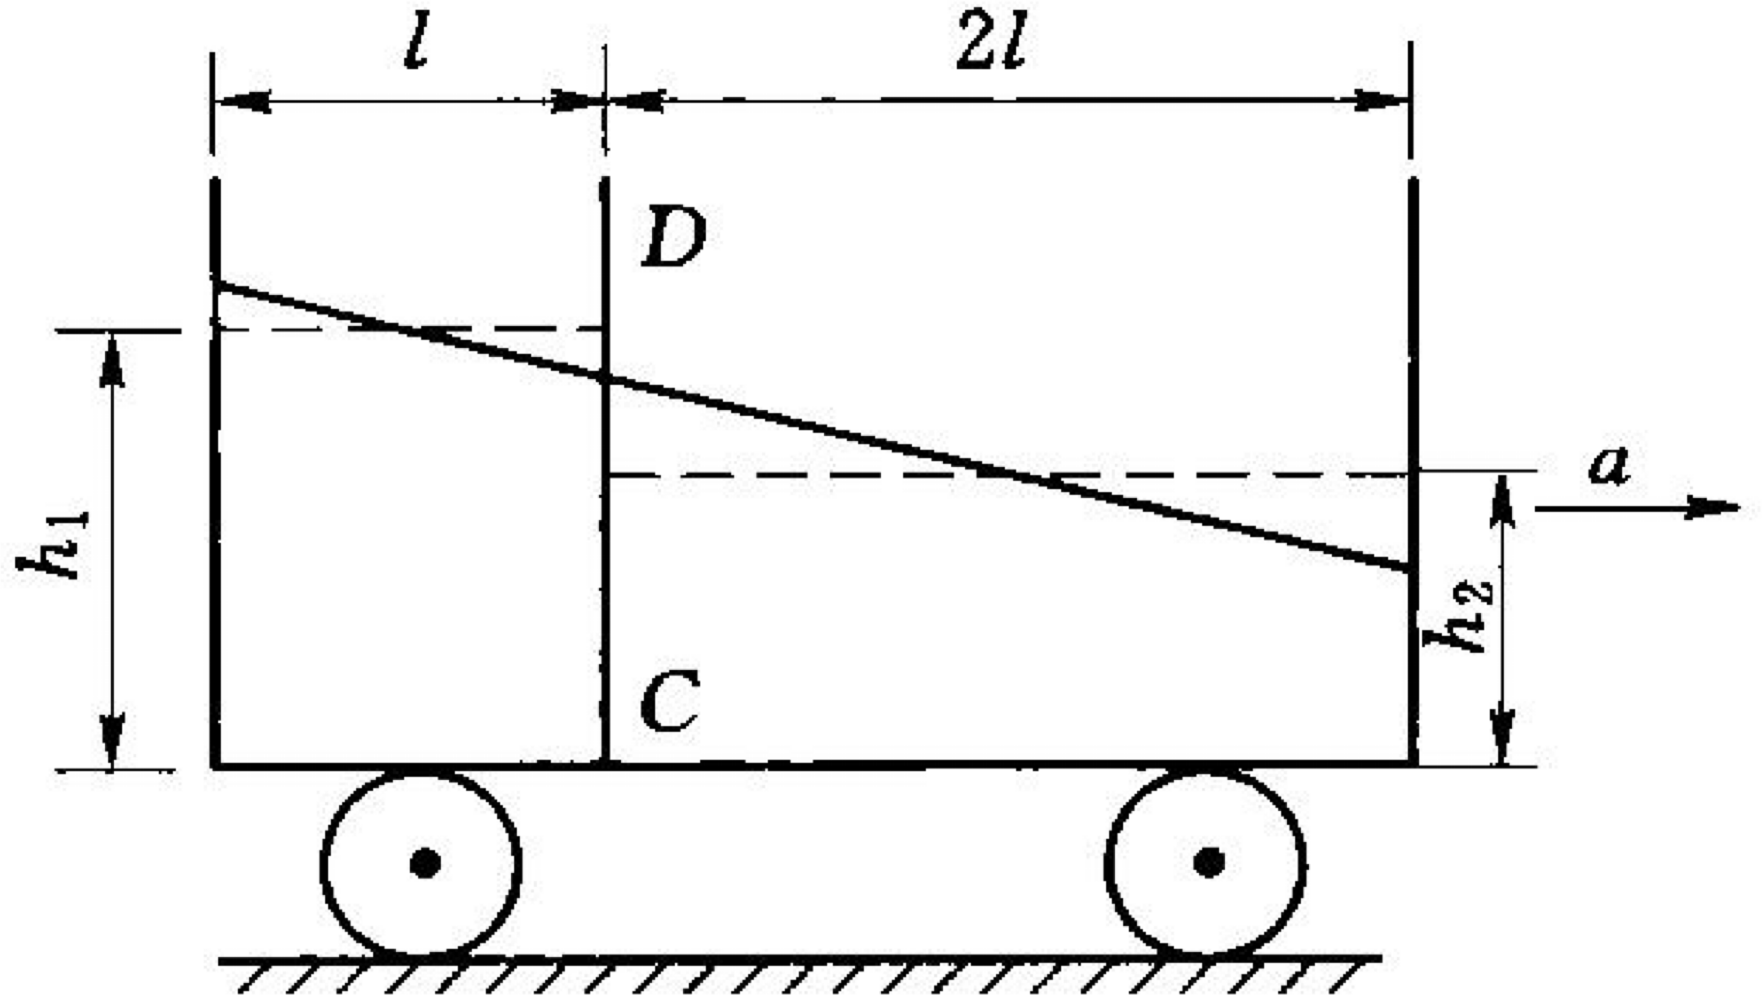
\includegraphics[width=0.7\textwidth,height=0.52\textheight,keepaspectratio]{slides_assets/fluid_deck01/accel-cart.png}\\
  {\scriptsize 图：源讲义原图}
  \end{center}
  \TLtakeaway{容器向右加速时，自由液面左高右低；斜率大小为 $a_x/g$。}
\end{frame}

\begin{frame}{重力加惯性力：等角速度旋转}
  容器绕竖直轴以角速度 $\omega$ 匀速旋转。随容器旋转的参考系中，单位质量离心惯性力为 $\omega^2r\,\vc e_r$，重力为 $-g\vc k$。
  \[
    \vc f=\omega^2r\,\vc e_r-g\vc k.
  \]
  沿轴对称截面移动，$\rd\vc r=\rd r\,\vc e_r+\rd z\,\vc k$，等压面满足
  \[
    \omega^2r\,\rd r-g\,\rd z=0.
  \]
  积分：
  \[
    \boxed{\frac{1}{2}\omega^2r^2-gz=C.} \tag{S12}
  \]
  改写为自由液面形状：
  \[
    \boxed{z=\frac{\omega^2r^2}{2g}+C'.} \tag{S13}
  \]
  \TLtakeaway{旋转静止液体的自由液面是抛物面；中心低、边壁高。}
\end{frame}

\begin{frame}{旋转抛物面：中心下降与边壁上升}
  抽象的式 (S13) 可以用截面图理解：离轴越远，离心惯性力越大，所以等压面必须向上抬高才能保持与有效质量力正交。
  \begin{center}
  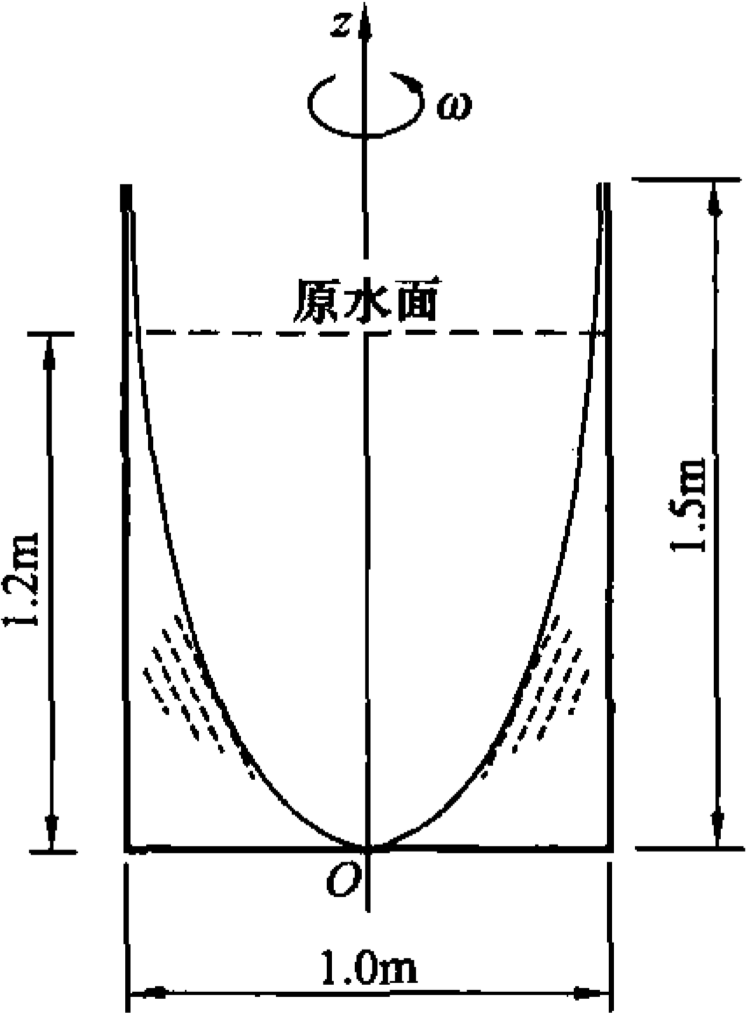
\includegraphics[width=0.7\textwidth,height=0.46\textheight,keepaspectratio]{slides_assets/fluid_deck01/rotation-parabola.png}\\
  {\scriptsize 图：源讲义原图}
  \end{center}
  \TLtakeaway{若未溢出，体积守恒决定抛物面常数；若已溢出，边壁液面被容器高度限制。}
\end{frame}

\begin{frame}{算例 S2（\#61）：旋转圆筒的状态判断}
  圆筒直径 $1\,\mathrm{m}$，半径 $R=0.5\,\mathrm{m}$；筒高 $H=1.5\,\mathrm{m}$；初始水深 $h_0=1.2\,\mathrm{m}$。旋转后筒底中心恰好无水。
  \begin{itemize}
    \item 中心恰好无水表示抛物面最低点在筒底：$z(0)=0$。
    \item 因此液面可写为
      \[
        z(r)=\frac{\omega^2r^2}{2g}.
      \]
    \item 若没有溢出，平均水深仍应为 $1.2\,\mathrm{m}$。抛物面从 $0$ 到边壁高度 $z_R$ 的平均高度是 $z_R/2$。
    \item 于是无溢出需要 $z_R=2h_0=2.4\,\mathrm{m}$，但筒高只有 $1.5\,\mathrm{m}$。
  \end{itemize}
  \TLtakeaway{本题一定发生溢水；最终边壁液面只能达到筒口高度 $H=1.5\,\mathrm{m}$。}
\end{frame}

\begin{frame}{算例 S2（\#61）：由边壁高度求角速度}
  由于发生溢水，最终抛物面经过筒底中心和筒口边缘：
  \[
    z(0)=0,\qquad z(R)=H=1.5\,\mathrm{m}.
  \]
  代入
  \[
    z(R)=\frac{\omega^2R^2}{2g}=H.
  \]
  解出角速度：
  \[
    \omega=\sqrt{\frac{2gH}{R^2}}.
  \]
  代入 $g=9.8\,\mathrm{m/s^2}$、$R=0.5\,\mathrm{m}$：
  \[
    \omega=\sqrt{\frac{2\times9.8\times1.5}{0.5^2}}
      \approx10.8\,\mathrm{rad/s}. \tag{S14}
  \]
  \TLtakeaway{旋转角速度由“中心刚露底”和“边壁到筒口”两个几何条件共同确定。}
\end{frame}

\begin{frame}{算例 S2（\#61）：由体积差求溢水量}
  初始水量为
  \[
    V_0=\pi R^2h_0=\pi(0.5)^2(1.2)=0.300\pi\,\mathrm{m^3}.
  \]
  最终水面是从中心 $0$ 到边壁 $H$ 的抛物面，其平均高度为 $H/2$，所以剩余水量为
  \[
    V_1=\pi R^2\frac{H}{2}
       =\pi(0.5)^2\frac{1.5}{2}
       =0.1875\pi\,\mathrm{m^3}.
  \]
  溢水量为
  \[
    V_{\mathrm{spill}}=V_0-V_1
      =0.1125\pi\approx0.353\,\mathrm{m^3}. \tag{S15}
  \]
  \TLtakeaway{先判断是否溢出，再决定用体积守恒还是筒口高度；这一步不能省。}
\end{frame}

\begin{frame}{平面上的静水总压力：为什么等于形心压强乘面积？}
  对任意平面受压面，压强沿某个坐标 $y$ 线性变化。这里 $y$ 从零压线沿平面向深处量，令
  \[
    p=\kappa y,
  \]
  其中垂直平面可取 $\kappa=\rho g$，倾斜平面可取 $\kappa=\rho g\sin\alpha$。
  总压力是压强在面积上的积分：
  \[
    P=\int_A p\,\rd A=\int_A \kappa y\,\rd A.
  \]
  形心坐标满足
  \[
    y_c=\frac{1}{A}\int_A y\,\rd A.
  \]
  代入上式：
  \[
    \boxed{P=\kappa y_c A=p_c A.} \tag{S16}
  \]
  \TLtakeaway{平面总压力大小只需要形心处压强 $p_c$ 和受压面积 $A$，但作用点一般不在形心。}
\end{frame}

\begin{frame}{压力中心：由“对零压线取矩”推导}
  \TLterm{压力中心}是总压力作用线穿过受压面的点。设它的坐标为 $y_D$。对零压线取矩，左边用合力，右边用分布力积分。\proofskipnote
  \[
    P y_D=\int_A y\,p\,\rd A.
  \]
  代入 $p=\kappa y$：
  \[
    P y_D=\kappa\int_A y^2\,\rd A.
  \]
  零压线轴的二次矩为
  \[
    I_0=\int_A y^2\,\rd A.
  \]
  平行轴定理给出
  \[
    I_0=I_c+y_c^2A,
  \]
  其中 $I_c$ 是关于过形心且平行于零压线轴的面积二次矩。
\end{frame}

\begin{frame}{压力中心公式：为什么总在形心更深处？}
  上一帧得到 $P y_D=\kappa I_0$，又由式 (S16) 知 $P=\kappa y_cA$。\proofskipnote
  两式相除：
  \[
    y_D=\frac{I_0}{y_cA}.
  \]
  代入 $I_0=I_c+y_c^2A$：
  \[
    \boxed{y_D=y_c+\frac{I_c}{y_cA}.} \tag{S17}
  \]
  因为 $I_c>0$、$y_c>0$、$A>0$，所以
  \[
    y_D>y_c.
  \]
  \TLtakeaway{下部压强更大，分布力矩把合力作用点拉到形心以下。}
\end{frame}

\begin{frame}{压力中心图像：合力被更深处拉下去}
  这张图只表达位置关系：形心 $c$ 是几何平均点，压力中心 $D$ 是压强加权后的合力作用点。
  \begin{center}
  \begin{tikzpicture}[scale=0.66,>={Stealth[length=5pt]}]
    \fill[TLprimaryTint] (-1.4,-1.2) rectangle (1.4,1.2);
    \draw[TLprimary,thick] (-1.4,-1.2) rectangle (1.4,1.2);
    \draw[TLaccent,thick] (-1.4,1.2)--(1.4,1.2) node[right]{零压线};
    \fill[TLprimaryDark] (0,0) circle (2pt) node[right]{形心 $c$};
    \fill[TLaccent] (0,-0.35) circle (2pt) node[right]{压力中心 $D$};
    \draw[->,TLaccent,thick] (1.9,1.0)--(1.9,-1.0) node[midway,right]{压强随深度增大};
  \end{tikzpicture}
  \end{center}
  \TLtakeaway{若受压面水平放置，各点压强相同，压力中心才会与形心重合。}
\end{frame}

\begin{frame}{矩形平面：用压强分布图求总压力}
  对宽度为 $b$ 的矩形平面，若沿长度 $L$ 的上、下端水深分别为 $h_1,h_2$，压强分布是一块梯形。
  \begin{columns}[T]
    \column{0.52\textwidth}
      \begin{itemize}
        \item 压强图面积记为 $\Omega$，单位为 $\mathrm{N/m}$。
        \item 总压力为
          \[
            \boxed{P=\Omega b.} \tag{S18}
          \]
        \item 合力作用线穿过压强图形心。
        \item 从深端下缘向上量的距离为
          \[
            \boxed{e=\frac{L(2h_1+h_2)}{3(h_1+h_2)}}. \tag{S19}
          \]
      \end{itemize}
    \column{0.48\textwidth}
      \centering
      \begin{tikzpicture}[scale=0.72,>={Stealth[length=5pt]}]
        \draw[TLprimary,thick] (0,-1.3) rectangle (0.28,1.3);
        \draw[TLaccent,thick,fill=TLaccentLight] (0.55,1.0)--(2.1,1.0)--(2.1,-1.0)--(0.55,-1.0)--cycle;
        \draw[TLaccent,thick] (0.55,1.0)--(1.25,-1.0);
        \draw[<->,TLinkSoft] (-0.25,1.0)--(-0.25,-1.0) node[midway,left]{$L$};
        \node[TLinkSoft] at (1.55,1.35) {$p_1=\rho gh_1$};
        \node[TLinkSoft] at (1.55,-1.35) {$p_2=\rho gh_2$};
        \draw[->,TLprimaryDark,thick] (1.35,-0.25)--(2.4,-0.25) node[right]{$P$};
      \end{tikzpicture}
  \end{columns}
  \TLtakeaway{矩形题可以把“积分”换成“压强图面积乘宽度”，但压力中心仍要取图形心。}
\end{frame}

\begin{frame}{算例 S3（\#64）：矩形闸门的已知量与总压力}
  已知矩形平板闸门长 $l=2\,\mathrm{m}$，宽 $b=1\,\mathrm{m}$，形心水深 $h_c=2\,\mathrm{m}$，倾角 $\alpha=45^\circ$，上缘 $A$ 为转轴。
  \[
    A=lb=2\,\mathrm{m^2}.
  \]
  总压力大小为
  \[
    P=\rho g h_cA
      =1000\times9.8\times2\times2
      =3.92\times10^4\,\mathrm{N}. \tag{S20}
  \]
  沿闸门量的形心坐标为
  \[
    y_c=\frac{h_c}{\sin45^\circ}=2.828\,\mathrm{m}.
  \]
  矩形关于形心轴的二次矩为
  \[
    I_c=\frac{bl^3}{12}=\frac{1\times2^3}{12}=0.667\,\mathrm{m^4}.
  \]
\end{frame}

\begin{frame}{算例 S3（\#64）：求压力中心到转轴距离}
  压力中心沿闸门的坐标为
  \[
    y_D=y_c+\frac{I_c}{y_cA}
      =2.828+\frac{0.667}{2.828\times2}
      =2.946\,\mathrm{m}.
  \]
  上缘转轴 $A$ 到零压线的沿面距离为
  \[
    y_A=y_c-\frac{l}{2}=2.828-1=1.828\,\mathrm{m}.
  \]
  因此压力中心到转轴的力臂为
  \[
    AD=y_D-y_A=1.118\,\mathrm{m}. \tag{S21}
  \]
  \begin{center}
  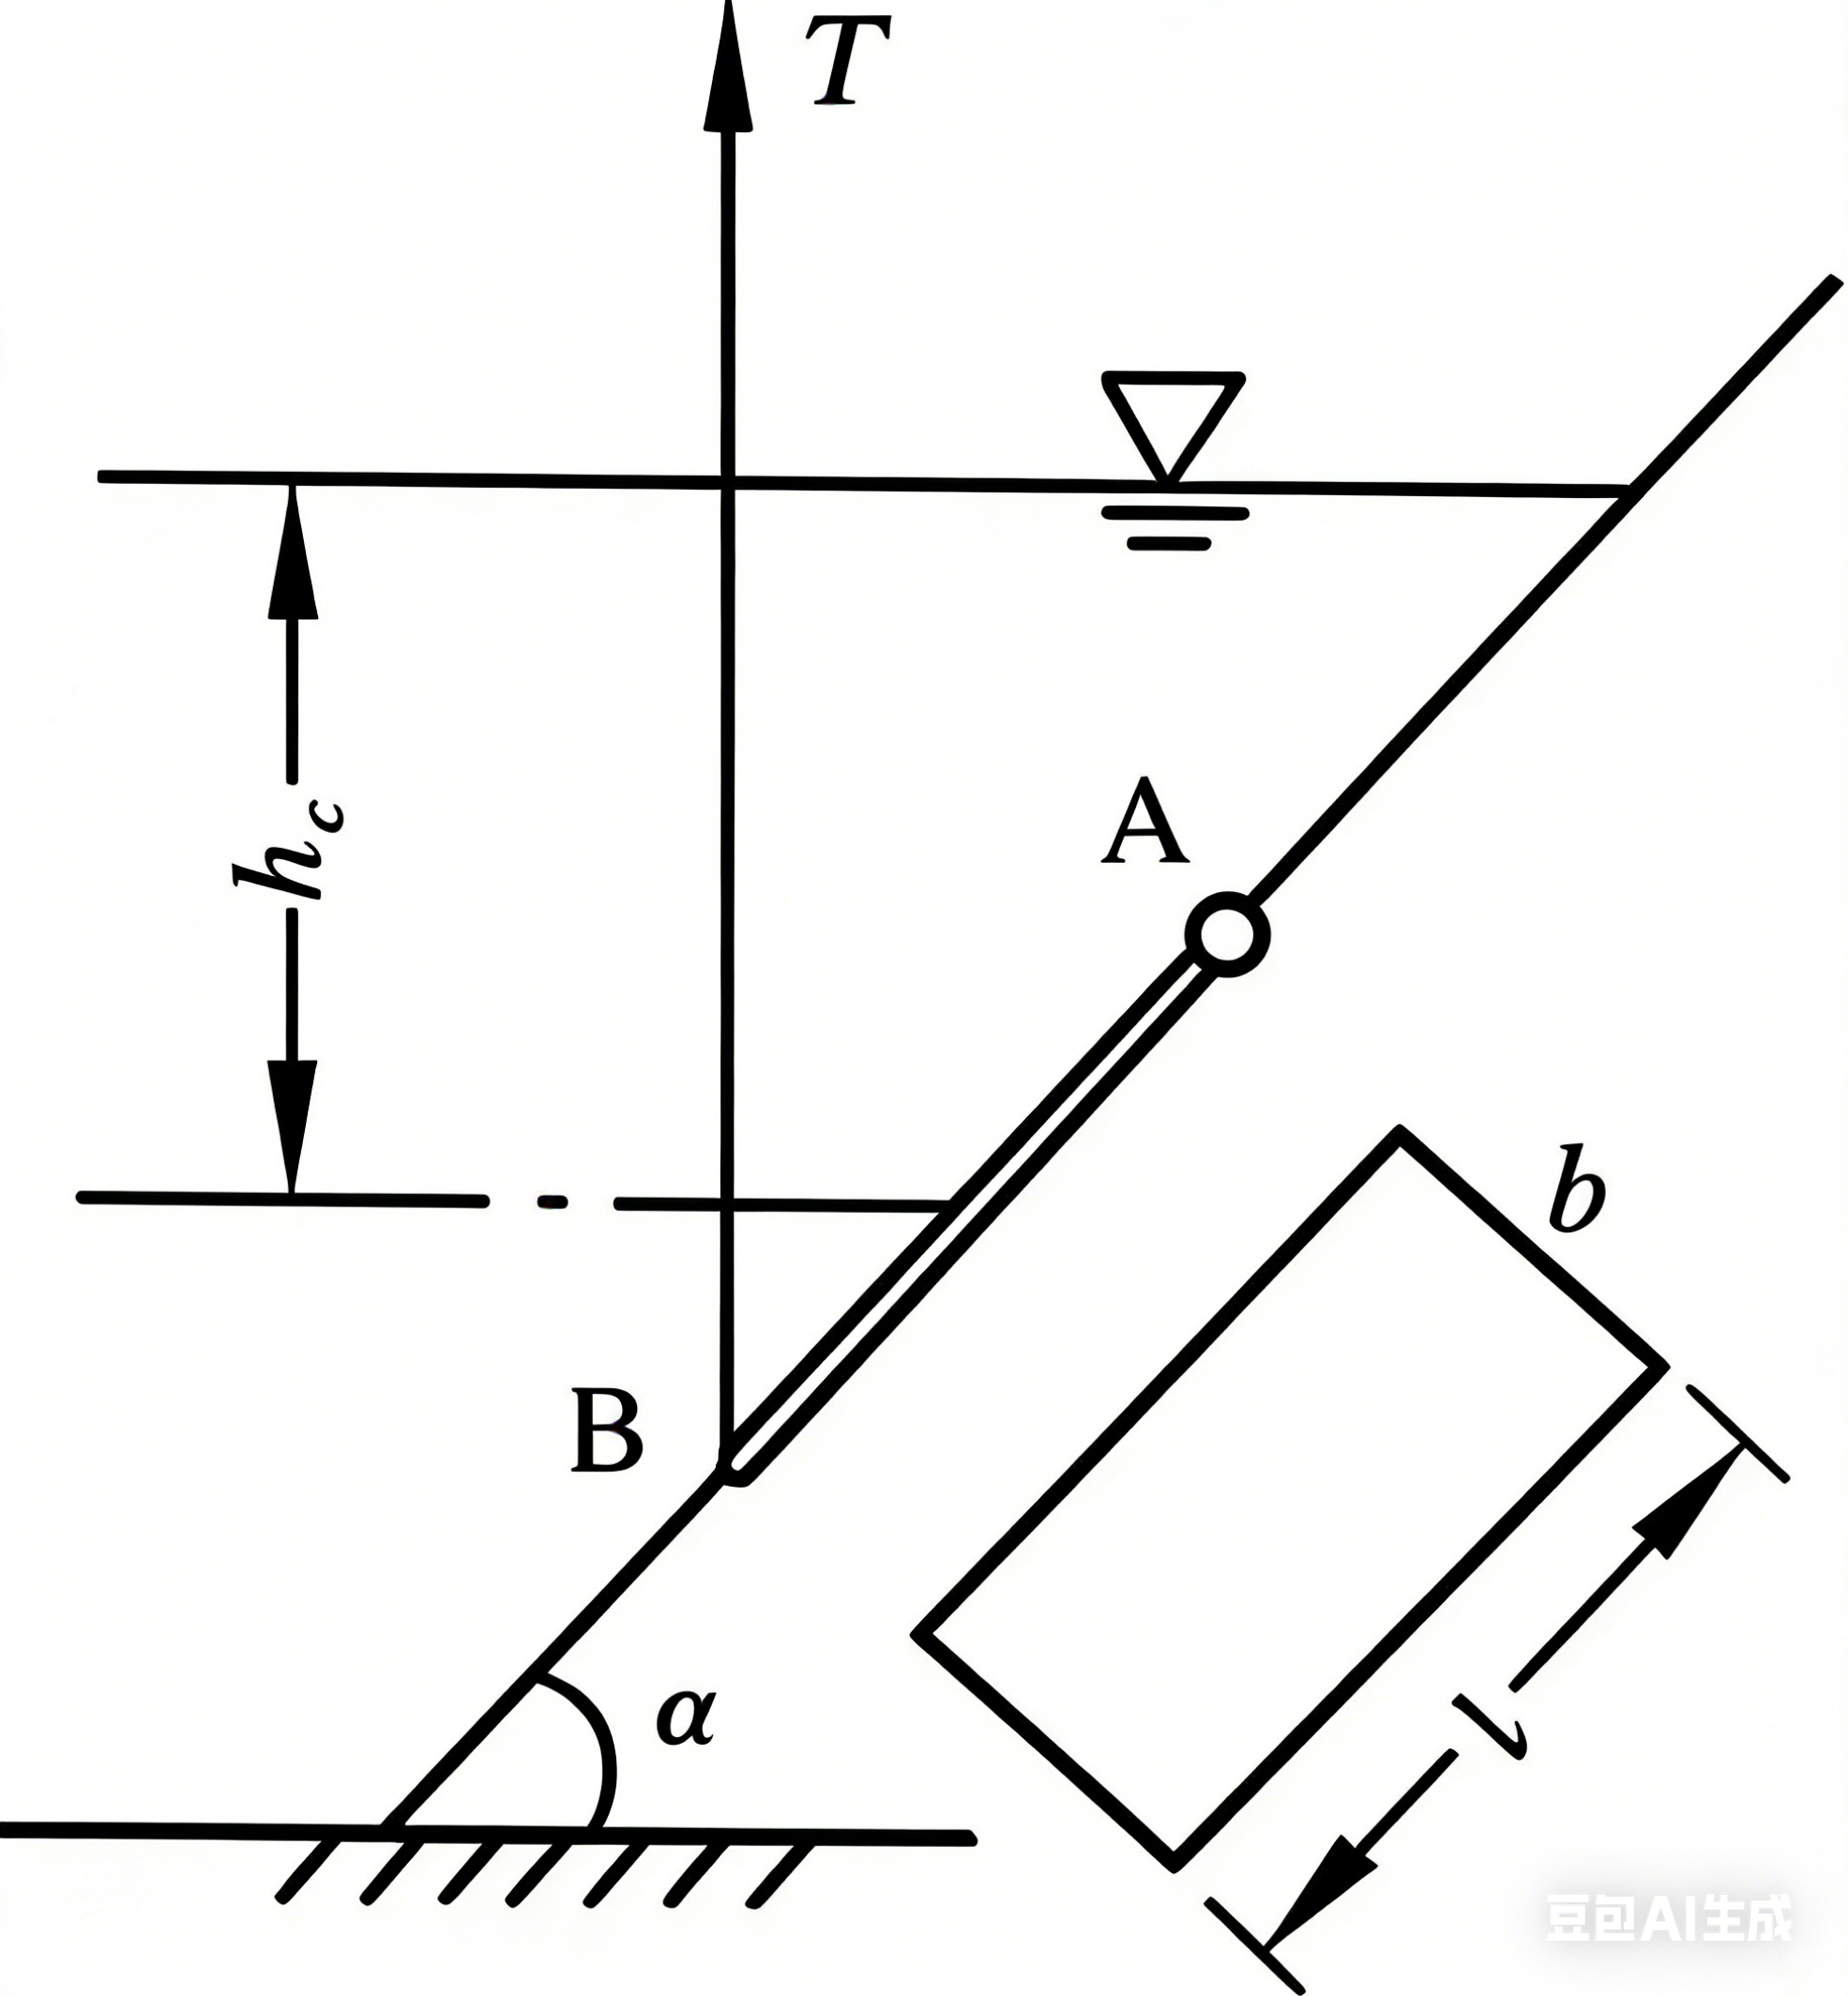
\includegraphics[width=0.7\textwidth,height=0.20\textheight,keepaspectratio]{slides_assets/fluid_deck01/ex-gate-incline.png}\\
  {\scriptsize 图：源讲义原图}
  \end{center}
\end{frame}

\begin{frame}{算例 S3（\#64）：由转轴取矩求拉力}
  忽略自重时，对转轴 $A$ 取矩。总压力 $P$ 垂直于闸门，力臂为 $AD$；竖直拉力 $T$ 作用在下缘，水平力臂为 $l\cos\alpha$。
  \[
    T\,l\cos\alpha=P\,AD.
  \]
  因此
  \[
    T=\frac{P\,AD}{l\cos45^\circ}
      =\frac{(3.92\times10^4)\times1.118}{2\times0.707}
      \approx3.10\times10^4\,\mathrm{N}.
  \]
  若闸门自重 $G=2000\,\mathrm{N}$ 不可忽略，重力作用于形心，关于 $A$ 的力臂为 $(l/2)\cos45^\circ$，且与水压力同向增大开门所需拉力：
  \[
    T=\frac{P\,AD+G(l/2)\cos45^\circ}{l\cos45^\circ}
      \approx3.20\times10^4\,\mathrm{N}. \tag{S22}
  \]
  \TLtakeaway{先求总压力和压力中心，再对转轴取矩；自重是否计入只改变力矩平衡式。}
\end{frame}

\begin{frame}{曲面总压力：先把向量问题拆成两个分量}
  曲面上每一点压强方向都沿局部法线，直接相加不方便。做题时先求\TLterm{水平分力}和\TLterm{铅直分力}，再合成总压力。
  \begin{columns}[T]
    \column{0.56\textwidth}
      水平分力等于该曲面在铅垂面上的投影面所受总压力：
      \[
        P_x=P_{\mathrm{proj}}
        =p_cA_{\mathrm{proj}}. \tag{S23}
      \]
      铅直分力等于\TLterm{压力体}内液体重量：
      \[
        P_z=\rho gV. \tag{S24}
      \]
      方向由压力体相对曲面的位置决定：压力体在曲面上方时，曲面对水的反力向上，水对曲面的力向下。
    \column{0.44\textwidth}
      \centering
      \begin{tikzpicture}[scale=0.78,>={Stealth[length=5pt]}]
        \fill[teal!10] (-1.9,-1.55) rectangle (0.8,1.15);
        \draw[teal!70!black,thick] (-1.9,1.15)--(0.8,1.15) node[right]{自由液面};
        \draw[teal!70!black,very thick] (0.0,-1.35) to[out=70,in=-70] (0.0,0.85);
        \draw[teal!70!black,dashed] (0.0,-1.35)--(0.0,0.85);
        \fill[teal!25,opacity=0.65] (0.0,-1.35) to[out=70,in=-70] (0.0,0.85)--(0.0,1.15)--cycle;
        \draw[->,teal!70!black,thick] (0.2,-0.2)--(1.25,-0.2) node[right]{$P_x$};
        \draw[->,teal!70!black,thick] (-0.35,-0.1)--(-0.35,-1.15) node[below]{$P_z$};
        \node[TLinkSoft] at (-1.05,-1.85) {水域};
        \node[TLinkSoft] at (0.85,0.45) {压力体};
      \end{tikzpicture}
  \end{columns}
  \TLtakeaway{曲面题的主线是“水平看投影，铅直看压力体”。}
\end{frame}

\begin{frame}{压力体：为什么铅直分力等于一块液体的重量}
  \proofskipnote
  设想把曲面、两侧铅直面和自由液面围成一个静止的液体体积。这个体积不是额外假设，而是为了把曲面压力换成一个可以平衡的力系。
  \begin{enumerate}
    \item 铅直侧面上的压强力水平作用，所以它们没有铅直分量。
    \item 自由液面用相对压强表示时 $p=0$，所以顶部没有相对压强合力。
    \item 剩下的铅直外力只有液体重力 $\rho gV$ 和曲面对这块液体的支持力。
  \end{enumerate}
  静止要求铅直方向合力为零，因此曲面对液体的力大小为 $\rho gV$；按作用反作用，液体对曲面的铅直分力大小也为
  \[
    P_z=\rho gV.
  \]
  \TLtakeaway{压力体法不是记忆技巧；它把曲面的铅直压力分量转化成一个静止液体体积的重量平衡。}
\end{frame}

\begin{frame}{曲面总压力：合力大小、方向和作用线}
  求出两个分力后，总压力由直角三角形合成：
  \[
    P=\sqrt{P_x^2+P_z^2},\qquad
    \alpha=\arctan\frac{P_z}{P_x}. \tag{S25}
  \]
  这里 $\alpha$ 是总压力作用线与水平线的夹角。作用线的定位按两步做：
  \begin{itemize}
    \item $P_x$ 的作用线通过铅垂投影面上总压力的压力中心；
    \item $P_z$ 的作用线通过压力体形心；
    \item 两条分力作用线的交点给出合力作用线，总压力作用线与曲面的交点就是曲面上的作用点。
  \end{itemize}
  \begin{center}
  \begin{tikzpicture}[scale=0.7,>={Stealth[length=5pt]}]
    \draw[teal!70!black,very thick] (-1.5,-0.9) to[out=45,in=-45] (-1.5,1.1);
    \draw[->,teal!70!black,thick] (-0.65,0.1)--(1.0,0.1) node[right]{$P_x$};
    \draw[->,teal!70!black,thick] (-0.65,0.1)--(-0.65,-1.15) node[below]{$P_z$};
    \draw[->,TLaccent,very thick] (-0.65,0.1)--(0.85,-1.05) node[right]{$P$};
    \draw[TLinkSoft] (-0.15,0.1) arc[start angle=0,end angle=-37,radius=0.5];
    \node[TLinkSoft] at (0.42,-0.2) {$\alpha$};
  \end{tikzpicture}
  \end{center}
\end{frame}

\begin{frame}{算例 S4（\#63）：半圆弧曲面的水平分力}
  题图由三个半圆弧连接而成，半径为 $R_3=3\,\mathrm{m}$、$R_2=2\,\mathrm{m}$、$R_1=1\,\mathrm{m}$，曲面宽 $b=2\,\mathrm{m}$，点 $A$ 在自由液面。
  \begin{columns}[T]
    \column{0.48\textwidth}
      \begin{center}
      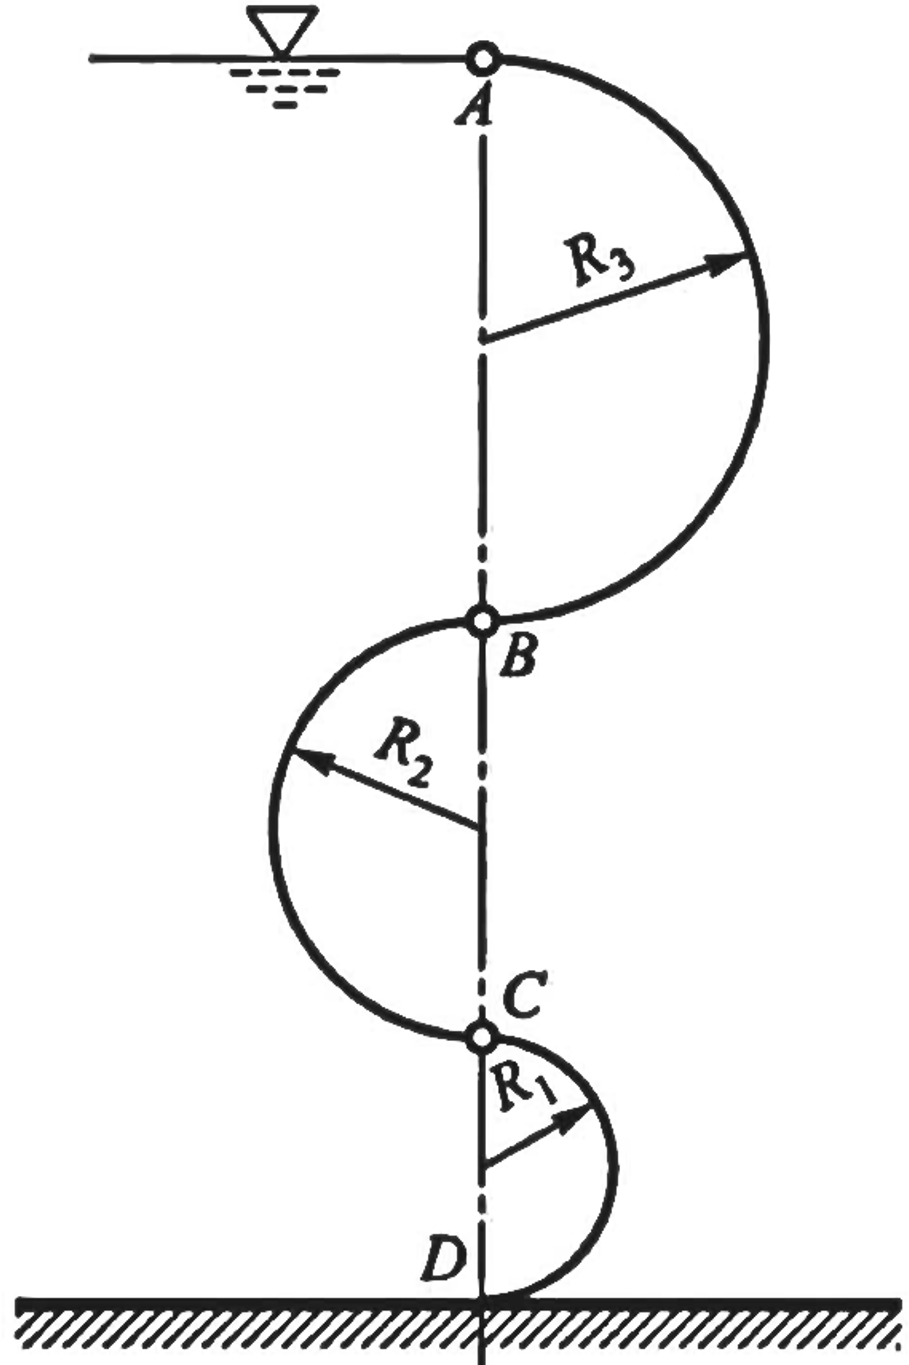
\includegraphics[width=\linewidth,height=0.48\textheight,keepaspectratio]{slides_assets/fluid_deck01/ex-curved-3arc.png}\\
      {\scriptsize 图：源讲义原图}
      \end{center}
    \column{0.52\textwidth}
      水平分力只看铅垂投影面。投影高度为 $H=2R_3+2R_2+2R_1=12\,\mathrm{m}$，面积为 $A_{\mathrm{proj}}=Hb=24\,\mathrm{m^2}$，形心水深为 $h_c=H/2=6\,\mathrm{m}$。所以
      \[
        \begin{aligned}
        P_x&=\rho gh_cA_{\mathrm{proj}}\\
           &=1000\times9.8\times6\times24\\
           &=1.411\times10^6\,\mathrm{N}.
        \end{aligned} \tag{S26}
      \]
  \end{columns}
\end{frame}

\begin{frame}{算例 S4（\#63）：压力体求铅直分力}
  三段半圆弧的压力体要带符号相加。向右凸的弧段贡献取正，向左凸的弧段贡献取负；本题为
  \[
    A_V=\frac{\pi}{2}\left(R_3^2-R_2^2+R_1^2\right)
       =\frac{\pi}{2}(9-4+1)
       =3\pi\,\mathrm{m^2}.
  \]
  曲面宽 $b=2\,\mathrm{m}$，压力体体积为
  \[
    V=A_Vb=6\pi\,\mathrm{m^3}.
  \]
  因此铅直分力大小为
  \[
    P_z=\rho gV=1000\times9.8\times6\pi
       =1.847\times10^5\,\mathrm{N}. \tag{S27}
  \]
  合力约为 $P=1.423\times10^6\,\mathrm{N}$，与水平线夹角 $\alpha=\arctan(P_z/P_x)\approx7.5^\circ$。按该符号压力体，铅直分力方向向下。
\end{frame}

\begin{frame}{压强分布图：先画基准，再画随深度线性增长}
  压强分布图回答的是“每个深度处单位面积被推多大”。画图时先定相对压强基准，再按水深画长度。
  \begin{columns}[T]
    \column{0.52\textwidth}
      \begin{itemize}
        \item 自由液面处相对压强为零。
        \item 同一种静止液体中，压强随深度线性增加。
        \item 不同密度液体中，斜率为 $\rho g$；密度越大，图线越陡。
        \item 两侧都有液体时，可先画两侧压强图，再抵消相同大小、相反方向的部分。
      \end{itemize}
    \column{0.48\textwidth}
      \centering
      \begin{tikzpicture}[scale=0.74,>={Stealth[length=5pt]}]
        \draw[teal!70!black,thick] (-1.0,1.3)--(1.0,1.3) node[right]{自由液面};
        \draw[teal!70!black,thick] (0,1.3)--(0,-1.5);
        \fill[teal!20] (0,1.3)--(1.35,-1.5)--(0,-1.5)--cycle;
        \draw[teal!70!black,very thick] (0,1.3)--(1.35,-1.5)--(0,-1.5);
        \draw[->,TLaccent,thick] (0,-0.65)--(0.95,-0.65);
        \node[TLinkSoft] at (0.95,-1.82) {$p=\rho gh$};
        \draw[<->,TLinkSoft] (-0.35,1.3)--(-0.35,-1.5) node[midway,left]{$h$};
      \end{tikzpicture}
  \end{columns}
  \TLtakeaway{压强图的长度表示压强大小；面积给出单位宽度上的总压力。}
\end{frame}

\begin{frame}{压力体绘制方法：同竖异横，竖下横上}
  压力体题先分段，再从每段曲线连到相应自由液面。源讲义给出的口诀可以这样用：
  \begin{itemize}
    \item “同竖异横”：曲线段与自由液面在同一竖向投影范围内时，直接竖向围成压力体；不在同一范围时，先水平延拓到自由液面所在区域。
    \item “竖下横上”：抵消压力体时，竖向围出的部分按向下压力保留，水平延拓形成的虚压力体按相反方向处理。
  \end{itemize}
  \begin{center}
  \begin{tikzpicture}[scale=0.72,>={Stealth[length=5pt]}]
    \draw[teal!70!black,thick] (-2.4,1.15)--(2.4,1.15) node[right]{自由液面};
    \draw[teal!70!black,very thick] (-1.5,-1.15) to[out=60,in=-90] (-0.25,0.4) to[out=90,in=210] (1.35,0.85);
    \fill[teal!18] (-1.5,-1.15) to[out=60,in=-90] (-0.25,0.4)--(-0.25,1.15)--(-1.5,1.15)--cycle;
    \fill[TLaccentLight,opacity=0.8] (-0.25,0.4) to[out=90,in=210] (1.35,0.85)--(1.35,1.15)--(-0.25,1.15)--cycle;
    \draw[teal!70!black,dashed] (-1.5,-1.15)--(-1.5,1.15);
    \draw[teal!70!black,dashed] (-0.25,0.4)--(-0.25,1.15);
    \draw[teal!70!black,dashed] (1.35,0.85)--(1.35,1.15);
    \node[TLinkSoft] at (-1.1,0.65) {竖向压力体};
    \node[TLinkSoft] at (0.35,1.58) {水平延拓体};
    \draw[->,TLaccent,thick] (-1.2,0.05)--(-1.2,-0.75) node[below]{向下};
    \draw[->,TLaccent,thick] (0.9,0.62)--(0.9,1.35)
      node[midway,right,fill=white,inner sep=1pt]{相反项};
  \end{tikzpicture}
  \end{center}
  \TLtakeaway{画压力体时不要先猜方向；先按自由液面围体，再用可抵消的虚实压力体判断净铅直分力。}
\end{frame}

\TLsection{常见误区}

\begin{frame}{常见误区：把适用条件说丢了}
  判断题最容易错的地方不是公式本身，而是把“静止”“运动”“基准”这些条件删掉。
  \TLwarnblock{三个条件型误区}{
    \begin{itemize}
      \item 说流体“不能承受剪切力”只在\TLterm{静止}时成立；运动中的黏性流体会用内摩擦力抵抗剪切变形。
      \item 说真空度“无上限”是错的；真空度最大只能等于当地大气压，标准大气压下约为 $101.325\,\mathrm{kPa}$。
      \item 说压力中心必与形心重合是错的；只有受压面水平、各点压强相同时，两者才重合。
    \end{itemize}
  }
  \[
    p_{\mathrm{vac}}=p_a-p_{\mathrm{abs}},\qquad 0\le p_{\mathrm{vac}}\le p_a .
  \]
  \TLtakeaway{判断一句话是否正确时，先问它有没有偷偷省略适用条件。}
\end{frame}

\begin{frame}{常见误区：把不同物理概念混成一个}
  有些错法来自“字面直觉”：看见大就以为容易，看见理想就以为什么都忽略。
  \TLwarnblock{两个概念型误区}{
    \begin{itemize}
      \item 体积弹性模量 $K$ 越大，流体越\TLterm{难}压缩，因为 $K=-\rd p/(\rd V/V)$ 表示单位体积相对缩小所需的压强增量。
      \item 理想流体不等于不可压缩流体；理想流体的定义是无黏，即 $\mu=0$，它是否可压缩要另行说明。
    \end{itemize}
  }
  \[
    \beta=\frac{1}{K},\qquad K\uparrow \Longleftrightarrow \beta\downarrow .
  \]
  \TLtakeaway{“无黏”“不可压缩”“静止”是三个不同标签，做题时不要自动捆绑。}
\end{frame}

\TLsection{练习}

\begin{frame}{练习 F1：油料的三个基本物性}
  \TLinfoblock{题目}{
    某油料密度为 $\rho=856\,\mathrm{kg/m^3}$。求该油料的相对密度 $s$、重度 $\gamma$ 和比体积 $v$。难度：$\star$。
  }
  \begin{itemize}
    \item 提示 1：相对密度以标准水的密度 $1000\,\mathrm{kg/m^3}$ 为基准。
    \item 提示 2：重度不是密度，需乘以 $g$，本讲义统一取 $g=9.8\,\mathrm{m/s^2}$。
    \item 提示 3：比体积是单位质量占有的体积，即 $v=1/\rho$。
  \end{itemize}
  \[
    s=\frac{\rho}{\rho_w},\qquad \gamma=\rho g,\qquad v=\frac{1}{\rho}.
  \]
  \TLtakeaway{同一个密度数据可以同时给出“相对重量感”“单位体积重量”和“单位质量体积”。}
\end{frame}

\begin{frame}{练习 F2：由动力黏度求运动黏度}
  \TLinfoblock{题目}{
    某液体的动力黏度为 $\mu=8.1\times10^{-2}\,\mathrm{Pa\cdot s}$，密度为 $\rho=0.79\times10^3\,\mathrm{kg/m^3}$。求运动黏度 $\nu$。难度：$\star$。
  }
  \begin{itemize}
    \item 提示 1：运动黏度把“黏”除以“密”，公式为 $\nu=\mu/\rho$。
    \item 提示 2：先把 $0.79\times10^3$ 写成 $790$，避免指数算错。
    \item 提示 3：单位应化为 $\mathrm{m^2/s}$。
  \end{itemize}
  \[
    [\nu]=\frac{\mathrm{kg/(m\cdot s)}}{\mathrm{kg/m^3}}=\mathrm{m^2/s}.
  \]
  \TLtakeaway{凡是把动力黏度换成运动黏度，都要同时检查数值和量纲。}
\end{frame}

\begin{frame}{练习 F3（\#30）：圆管抛物线速度分布的切应力}
  \TLinfoblock{题目}{
    圆管半径为 $R$，轴向流速分布为 $u=U_0(1-r^2/R^2)$。求切应力分布 $\tau(r)$，并给出管壁处切应力。难度：$\star\star$。
  }
  \begin{center}
  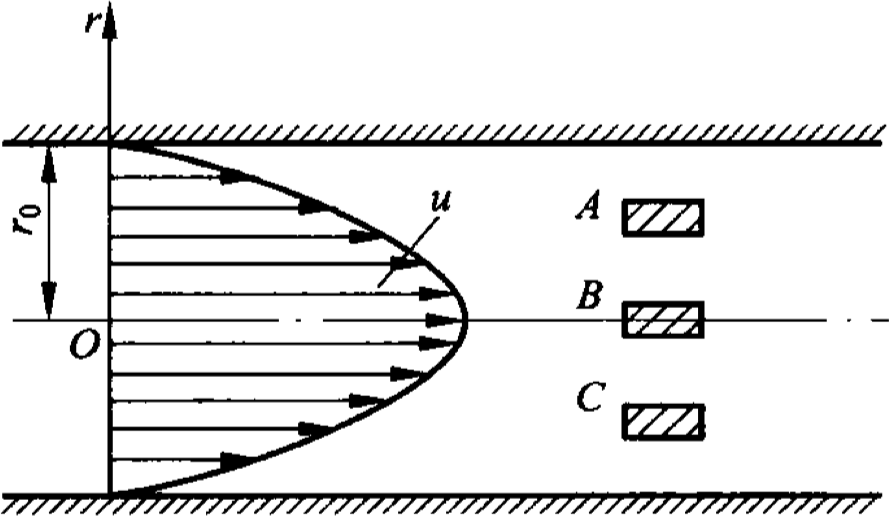
\includegraphics[width=0.30\textwidth,height=0.07\textheight,keepaspectratio]{slides_assets/fluid_deck01/ex-pipe-parabola.png}\\
  {\scriptsize 图：源讲义原图}
  \end{center}
  \begin{itemize}
    \item 提示 1：圆管中速度沿半径 $r$ 变化，所以先求 $\rd u/\rd r$。
    \item 提示 2：牛顿内摩擦定律给出切应力与速度梯度成正比。
    \item 提示 3：若只报阻碍流动的大小，取 $|\mu\,\rd u/\rd r|$。
  \end{itemize}
  \[
    \frac{\rd u}{\rd r}=-\frac{2U_0r}{R^2}.
  \]
  \TLtakeaway{抛物线速度剖面对应线性切应力分布，中心为零，管壁最大。}
\end{frame}

\begin{frame}{练习 F4（\#34）：圆锥旋转的黏性阻力矩}
  \TLinfoblock{题目}{
    圆锥绕中心轴以角速度 $\omega$ 旋转，锥顶半角为 $\alpha$，锥面与固定壁间隙为 $\delta$，油的动力黏度为 $\mu$，锥面母线长为 $L$。求阻力矩 $M$。难度：$\star\star\star$。
  }
  \begin{center}
  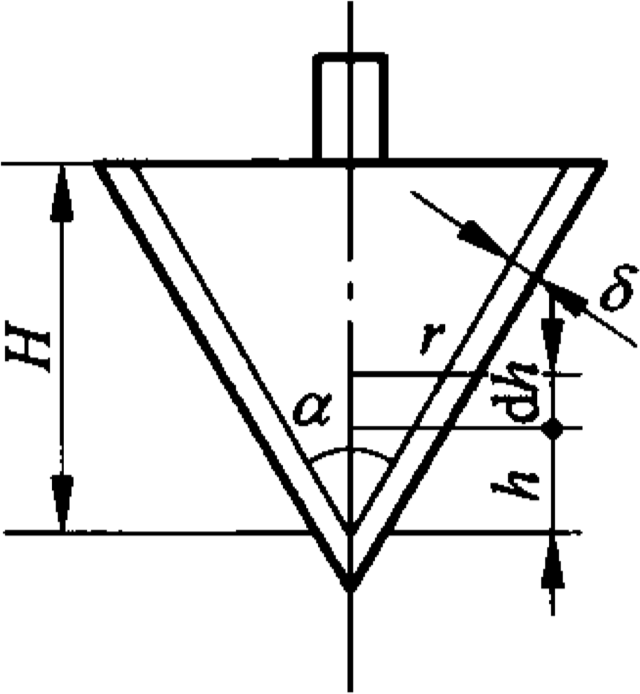
\includegraphics[width=0.30\textwidth,height=0.08\textheight,keepaspectratio]{slides_assets/fluid_deck01/ex-cone.png}\\
  {\scriptsize 图：源讲义原图}
  \end{center}
  \begin{itemize}
    \item 提示 1：取距锥顶母线长度为 $\ell$ 的微小环带，半径 $r=\ell\sin\alpha$。
    \item 提示 2：环带表面速度为 $\omega r$，近似速度梯度为 $\omega r/\delta$。
    \item 提示 3：微元阻力矩为 $\rd M=\tau\,\rd A\,r$，其中 $\rd A=2\pi r\,\rd\ell$。
  \end{itemize}
  \[
    \rd M=\frac{\mu\omega r}{\delta}\,(2\pi r\,\rd\ell)\,r .
  \]
  \TLtakeaway{旋转曲面题的关键是选环带微元；力矩比力多乘一个力臂 $r$。}
\end{frame}

\begin{frame}{练习 F5：密闭水箱底部表压与真空度}
  \TLinfoblock{题目}{
    密闭水箱顶部水面处表压为 $p_0=-20\,\mathrm{kPa}$，水深 $h=2\,\mathrm{m}$。求箱底表压和箱底真空度。难度：$\star$。
  }
  \begin{itemize}
    \item 提示 1：表压也可以直接使用静水压强公式，只要同一题中基准一致。
    \item 提示 2：向下深 $h$，表压增加 $\rho gh$。
    \item 提示 3：若底部表压仍为负，真空度等于它的绝对值。
  \end{itemize}
  \[
    p_{\mathrm{bottom},g}=p_{0,g}+\rho gh .
  \]
  \TLtakeaway{负表压不是错误，而是在说该点绝对压强低于当地大气压。}
\end{frame}

\begin{frame}{练习 F6（\#59）：轻油与重油的深度和测压管高度}
  \TLinfoblock{题目}{
    圆柱形油桶总高 $5\,\mathrm{m}$，上层轻油密度 $\rho_1=600\,\mathrm{kg/m^3}$，下层重油密度 $\rho_2=900\,\mathrm{kg/m^3}$。两种油重量相等，求 $h_1,h_2$，并求两根测压管内油面从桶底算起的高度。难度：$\star\star$。
  }
  \begin{center}
  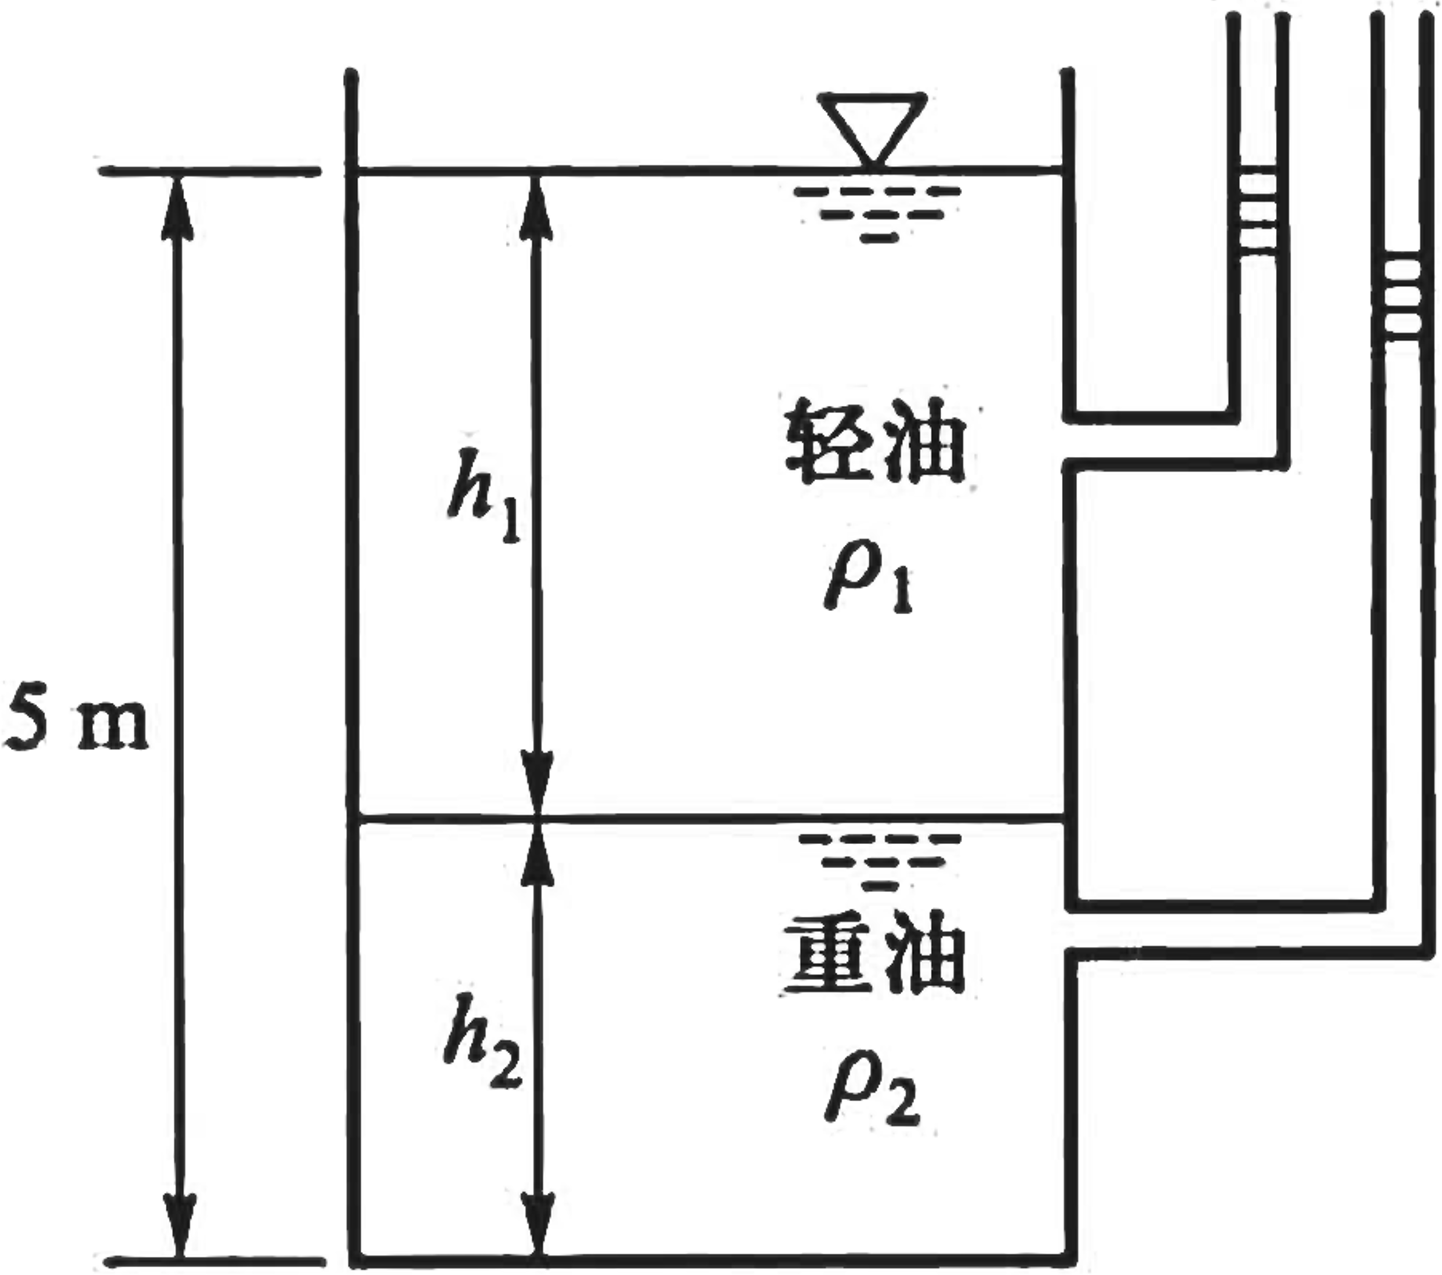
\includegraphics[width=0.24\textwidth,height=0.03\textheight,keepaspectratio]{slides_assets/fluid_deck01/ex-oil-2layer.png}\\[-1pt]
  {\scriptsize 图：源讲义原图}
  \end{center}
  \begin{itemize}
    \item 提示 1：同一圆柱桶中，两层油横截面积相同，重量相等可写成 $\rho_1 h_1=\rho_2 h_2$。
    \item 提示 2：总高度给出 $h_1+h_2=5\,\mathrm{m}$。
    \item 提示 3：接轻油层的测压管与桶内自由液面同高；接桶底重油的测压管用重油压强水头换算。
  \end{itemize}
  \[
    \rho_1 h_1=\rho_2h_2,\qquad h_1+h_2=5 .
  \]
  \TLtakeaway{分层液体题先写界面处压强连续，再按测压管中实际液体的密度换算高度。}
\end{frame}

\begin{frame}{练习 F7（\#62）：圆形放水孔的总压力与压力中心}
  \TLinfoblock{题目}{
    渠道侧壁开有圆形放水孔，孔径 $d=1\,\mathrm{m}$，孔顶至自由液面的深度为 $3\,\mathrm{m}$。求闸门所受总压力 $F$ 和压力中心深度 $h_D$。难度：$\star\star$。
  }
  \begin{itemize}
    \item 提示 1：圆孔形心水深为 $h_c=3+d/2$。
    \item 提示 2：平面静水总压力大小为 $F=\rho g h_c A$。
    \item 提示 3：竖直圆面压力中心深度为 $h_D=h_c+I_c/(h_cA)$。
  \end{itemize}
  \[
    A=\frac{\pi d^2}{4},\qquad I_c=\frac{\pi d^4}{64}.
  \]
  \TLtakeaway{压力中心比形心更深，因为下部压强更大，对力矩贡献更强。}
\end{frame}

\begin{frame}{练习 F8（\#69）：两侧水位同升时闸门合力增大}
  \TLinfoblock{题目}{
    倾斜平面闸门将两侧水隔开，左侧水位高于右侧。证明：两侧水位都上升相同高度 $\Delta h>0$ 后，闸门上的净静水总压力增大。难度：$\star\star\star$。
  }
  \begin{center}
  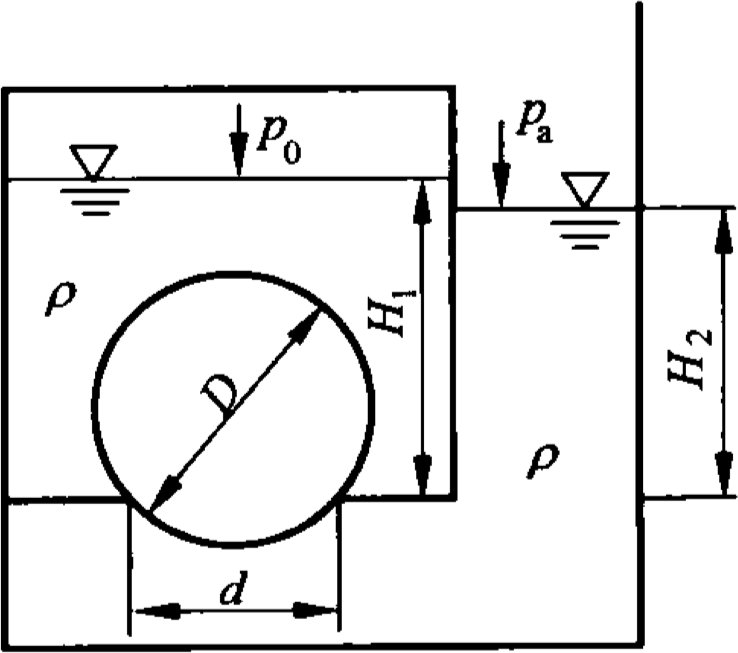
\includegraphics[width=0.30\textwidth,height=0.10\textheight,keepaspectratio]{slides_assets/fluid_deck01/ex-gate-2side.png}\\
  {\scriptsize 图：源讲义原图}
  \end{center}
  \begin{itemize}
    \item 提示 1：把两侧水深分别记为 $h_1>h_2$，闸门宽为 $b$，闸门与水平面的夹角为 $\alpha$。
    \item 提示 2：一侧三角形压强分布的总压力为 $\rho g b h^2/(2\sin\alpha)$。
    \item 提示 3：比较 $(h_1+\Delta h)^2-(h_2+\Delta h)^2$ 与 $h_1^2-h_2^2$。
  \end{itemize}
  \[
    (h_1+\Delta h)^2-(h_2+\Delta h)^2
    =(h_1^2-h_2^2)+2\Delta h(h_1-h_2).
  \]
  \TLtakeaway{两侧同升不改变水深差，但会放大“深水侧平方项”的优势。}
\end{frame}

\TLsection{延伸与文献注记}

\begin{frame}{本章对应讲义与阅读范围}
  本讲义外部资源仅供深化，不阅读外部资料也能完整掌握本讲义内容。
  \begin{center}
  \vspace{4pt}
  \small
  \begin{tabular}{@{}l l l@{}}
    \toprule
    \textbf{本讲义部分} & \textbf{源讲义章节} & \textbf{核心问题} \\
    \midrule
    第一章 & 流体基本物理概念 & 流体是什么，黏度、密度、压缩性怎样度量 \\
    第二章 & 水静力学 & 静水压强如何分布，平面和曲面受力怎样计算 \\
    练习与附录 & 两章习题 & 把概念换成可复算的工程数值 \\
    \bottomrule
  \end{tabular}
  \end{center}
  \[
    \text{物性} \longrightarrow \text{压强分布} \longrightarrow \text{静水总压力}.
  \]
  \TLtakeaway{本 deck 的目标是建立第一、二章的最小闭环：会解释、会计算、会检查量纲。}
\end{frame}

\begin{frame}{经典教材推荐：按使用层次选择}
  \begin{center}
  \vspace{4pt}
  \footnotesize
  \begin{tabular}{@{}l l l@{}}
    \toprule
    \textbf{教材} & \textbf{层次} & \textbf{特色} \\
    \midrule
    闻德荪《水力学》（上册） & 本科水力学 & 概念和工程题型贴近国内课程 \\
    吴持恭《水力学》 & 本科到考研 & 例题系统，静水压力题型覆盖细 \\
    White, \emph{Fluid Mechanics}, 8th ed. & 工程流体力学 & 物理图像清楚，量纲分析和应用强 \\
    Munson et al., \emph{Fundamentals of Fluid Mechanics} & 入门到进阶 & 例题丰富，适合补英文术语和工程语境 \\
    \bottomrule
  \end{tabular}
  \end{center}
  \[
    \text{先用中文教材巩固题型，再用英文教材对齐国际术语。}
  \]
  \TLtakeaway{外部教材的作用是扩展视野，不是替代本讲义的主线。}
\end{frame}

\begin{frame}{工程应用：静水压强不是纸面公式}
  \begin{columns}[T]
    \column{0.52\textwidth}
      \begin{itemize}
        \item 大坝和闸门设计：核心是 $F=p_cA$ 与压力中心位置。
        \item 水泵吸水：吸入口真空过大时，局部绝对压强可能低于汽化压强，引发空化和汽蚀。
        \item 帕斯卡液压机：小活塞压强传递到大活塞，用面积比放大力。
      \end{itemize}
    \column{0.48\textwidth}
      \centering
      \begin{tikzpicture}[scale=0.72,>={Stealth[length=5pt]}]
        \draw[teal!70!black,thick] (-1.8,1.0)--(1.8,1.0) node[right]{水面};
        \draw[teal!70!black,very thick] (-0.6,1.0)--(-0.6,-1.4);
        \fill[teal!18] (-0.6,1.0)--(1.2,-1.4)--(-0.6,-1.4)--cycle;
        \draw[->,TLaccent,thick] (-0.45,0.45)--(0.35,0.45);
        \draw[->,TLaccent,thick] (-0.45,-0.3)--(0.75,-0.3);
        \draw[->,TLaccent,thick] (-0.45,-1.05)--(1.1,-1.05);
        \node[TLinkSoft] at (0.75,-1.65) {$p=\rho gh$};
      \end{tikzpicture}
  \end{columns}
  \TLtakeaway{水静力学的工程价值在于把“哪里压得更大”转成“合力多大、作用线在哪里”。}
\end{frame}

\begin{frame}{人物简介：三条主线对应三位奠基者}
  \begin{center}
  \vspace{4pt}
  \footnotesize
  \begin{tabular}{@{}l l l@{}}
    \toprule
    \textbf{人物} & \textbf{本章相关概念} & \textbf{一句话联系} \\
    \midrule
    帕斯卡 Pascal & Pascal's principle & 封闭静止液体把外加压强等值传递到各处 \\
    牛顿 Newton & Newton's law of viscosity & 牛顿流体中切应力与速度梯度成正比 \\
    欧拉 Euler & Euler equation of hydrostatics & 平衡微分方程把压强梯度与质量力联系起来 \\
    \bottomrule
  \end{tabular}
  \end{center}
  \[
    \tau=\mu\frac{\rd u}{\rd y},\qquad
    \grad p=\rho\vc f,\qquad
    p=p_0+\rho(W-W_0).
  \]
  \TLtakeaway{历史名字不是背诵点，而是帮助你把“黏性”“静压传递”“平衡方程”分清楚。}
\end{frame}

\TLsection{术语速查}

\begin{frame}{术语速查（一）：流体物性与压强基础}
  \begin{center}
  \vspace{4pt}
  \footnotesize
  \setlength{\tabcolsep}{3pt}
  \begin{tabular}{@{}l l c l@{}}
    \toprule
    \textbf{中文} & \textbf{English} & \textbf{记号} & \textbf{一句话含义} \\
    \midrule
    粘度 & viscosity & $\mu$ & 抵抗剪切变形的强弱 \\
    运动粘度 & kinematic viscosity & $\nu$ & 动力黏度除以密度 \\
    重度 & specific weight & $\gamma$ & 单位体积流体的重量 \\
    相对密度 & relative density & $s$ & 与标准水密度的比值 \\
    体积模量 & bulk modulus & $K$ & 单位相对压缩所需压强 \\
    单位质量力 & body force per mass & $\vc f$ & 单位质量流体受的体积力 \\
    静水压强 & hydrostatic pressure & $p$ & 静止流体内部的法向压应力 \\
    等压面 & isobaric surface & -- & 压强处处相等的面 \\
    \bottomrule
  \end{tabular}
  \end{center}
  \TLtakeaway{第一组术语回答“流体有什么物性、静止时内部压强怎样描述”。}
\end{frame}

\begin{frame}{术语速查（二）：压强基准与静水总压力}
  \begin{center}
  \vspace{4pt}
  \footnotesize
  \setlength{\tabcolsep}{3pt}
  \begin{tabular}{@{}l l c l@{}}
    \toprule
    \textbf{中文} & \textbf{English} & \textbf{记号} & \textbf{一句话含义} \\
    \midrule
    测压管水头 & piezometric head & $z+p/(\rho g)$ & 单位重量液体的总势能 \\
    表压 & gauge pressure & $p_g$ & 相对当地大气压的压强 \\
    真空度 & vacuum & $p_{\mathrm{vac}}$ & 低于当地大气压的差值 \\
    绝对压强 & absolute pressure & $p_{\mathrm{abs}}$ & 以绝对真空为零点的压强 \\
    压力体（压体） & pressure body & $V$ & 曲面铅直分力对应的液体体积 \\
    形心 & centroid & $C$ & 面积的几何中心 \\
    压力中心 & center of pressure & $D$ & 静水总压力作用线穿过的点 \\
    \bottomrule
  \end{tabular}
  \end{center}
  \TLtakeaway{第二组术语回答“压强以谁为零点、合力作用在什么位置”。}
\end{frame}

\appendix

\begin{frame}{附录：练习 F1 全解}
  本题要从密度出发，分别计算三个派生物理量。
  \[
    \rho_w=1000\,\mathrm{kg/m^3}. \tag{A1}
  \]
  \[
    s=\frac{\rho}{\rho_w}=\frac{856}{1000}=0.856. \tag{A2}
  \]
  \[
    \gamma=\rho g=856\times9.8=8388.8\,\mathrm{N/m^3}
    =8.389\,\mathrm{kN/m^3}. \tag{A3}
  \]
  \[
    v=\frac{1}{\rho}=\frac{1}{856}=1.168\times10^{-3}\,\mathrm{m^3/kg}. \tag{A4}
  \]
  \TLresultblock{答案}{
    \[
      \boxed{s=0.856,\quad \gamma=8.389\,\mathrm{kN/m^3},\quad
      v=1.168\times10^{-3}\,\mathrm{m^3/kg}.}
    \]
  }
\end{frame}

\begin{frame}{附录：练习 F2 全解}
  本题要把动力黏度除以密度，得到运动黏度。
  \[
    \rho=0.79\times10^3=790\,\mathrm{kg/m^3}. \tag{A5}
  \]
  \[
    \nu=\frac{\mu}{\rho}. \tag{A6}
  \]
  \[
    \nu=\frac{8.1\times10^{-2}}{790}
       =1.025\times10^{-4}\,\mathrm{m^2/s}. \tag{A7}
  \]
  量纲检查为
  \[
    \frac{\mathrm{Pa\cdot s}}{\mathrm{kg/m^3}}
    =\frac{\mathrm{kg/(m\cdot s)}}{\mathrm{kg/m^3}}
    =\mathrm{m^2/s}. \tag{A8}
  \]
  \TLresultblock{答案}{
    \[
      \boxed{\nu=1.03\times10^{-4}\,\mathrm{m^2/s}.}
    \]
  }
\end{frame}

\begin{frame}{附录：练习 F3 全解}
  \small
  本题要把速度剖面的径向梯度转成切应力分布。
  \begin{align}
    u(r)&=U_0\left(1-\frac{r^2}{R^2}\right), \tag{A9}\\
    \frac{\rd u}{\rd r}
      &=U_0\left(-\frac{2r}{R^2}\right)
       =-\frac{2U_0r}{R^2}. \tag{A10}
  \end{align}
  按 $\tau_{rz}=\mu\,\rd u/\rd r$ 的符号约定，有
  \begin{align}
    \tau_{rz}(r)&=-\frac{2\mu U_0}{R^2}\,r, \tag{A11}\\
    |\tau(r)|&=\frac{2\mu U_0}{R^2}\,r,\qquad
    |\tau_w|=\frac{2\mu U_0}{R}. \tag{A12}
  \end{align}
  \TLresultblock{答案}{
    \(\boxed{\tau_{rz}(r)=-2\mu U_0r/R^2}\)，\(\boxed{|\tau_w|=2\mu U_0/R}\)。
  }
\end{frame}

\begin{frame}{附录：练习 F4 全解}
  本题要把锥面分成许多环带，再对阻力矩积分。
  \[
    r=\ell\sin\alpha,\qquad 0\le \ell\le L. \tag{A13}
  \]
  \[
    u=\omega r,\qquad
    \tau=\mu\frac{u}{\delta}=\frac{\mu\omega r}{\delta}. \tag{A14}
  \]
  \[
    \rd A=2\pi r\,\rd\ell. \tag{A15}
  \]
  \[
    \rd M=\tau\,\rd A\,r
    =\frac{2\pi\mu\omega}{\delta}r^3\,\rd\ell. \tag{A16}
  \]
  \[
    M=\int_0^L\frac{2\pi\mu\omega}{\delta}
       (\ell\sin\alpha)^3\,\rd\ell
     =\frac{\pi\mu\omega L^4\sin^3\alpha}{2\delta}. \tag{A17}
  \]
  \TLresultblock{答案}{
    \[
      \boxed{M=\dfrac{\pi\mu\omega L^4\sin^3\alpha}{2\delta}.}
    \]
  }
\end{frame}

\begin{frame}{附录：练习 F5 全解}
  本题要在表压基准下使用静水压强公式。
  \[
    p_{0,g}=-20\,\mathrm{kPa}. \tag{A18}
  \]
  \[
    \rho gh=1000\times9.8\times2
    =19600\,\mathrm{Pa}=19.6\,\mathrm{kPa}. \tag{A19}
  \]
  \[
    p_{\mathrm{bottom},g}
    =p_{0,g}+\rho gh
    =-20+19.6
    =-0.4\,\mathrm{kPa}. \tag{A20}
  \]
  底部表压仍为负，所以底部真空度为
  \[
    p_{\mathrm{vac}}=0.4\,\mathrm{kPa}
    =\frac{400}{1000\times9.8}=0.0408\,\mathrm{mH_2O}. \tag{A21}
  \]
  \TLresultblock{答案}{
    \[
      \boxed{p_{\mathrm{bottom},g}=-0.4\,\mathrm{kPa},\qquad
      p_{\mathrm{vac}}=0.4\,\mathrm{kPa}.}
    \]
  }
\end{frame}

\begin{frame}{附录：练习 F6 全解}
  \small
  本题先由重量相等求两层油深，再求测压管读数。
  \begin{align}
    h_1+h_2&=5, \tag{A22}\\
    \rho_1gh_1A&=\rho_2gh_2A
      \quad\Longrightarrow\quad 600h_1=900h_2, \tag{A23}\\
    h_1&=3\,\mathrm{m},\qquad h_2=2\,\mathrm{m}. \tag{A24}
  \end{align}
  接轻油层的开口测压管与桶内自由液面相通，所以油面高度为
  \[
    H_1=h_1+h_2=5\,\mathrm{m}. \tag{A25}
  \]
  接桶底重油的开口测压管满足
  \[
    \rho_2gH_2=\rho_1gh_1+\rho_2gh_2
    \quad\Longrightarrow\quad
    H_2=2+\frac{600}{900}\times3=4\,\mathrm{m}. \tag{A26}
  \]
  \TLresultblock{答案}{
    \(\boxed{h_1=3\,\mathrm{m},\ h_2=2\,\mathrm{m}}\)，
    \(\boxed{H_1=5\,\mathrm{m},\ H_2=4\,\mathrm{m}}\)。
  }
\end{frame}

\begin{frame}{附录：练习 F7 全解}
  本题是竖直圆形平面上的静水总压力。
  \[
    h_c=3+\frac{d}{2}=3.5\,\mathrm{m}. \tag{A27}
  \]
  \[
    A=\frac{\pi d^2}{4}
     =\frac{\pi}{4}
     =0.7854\,\mathrm{m^2}. \tag{A28}
  \]
  \[
    F=\rho gh_cA
     =1000\times9.8\times3.5\times0.7854
     =2.694\times10^4\,\mathrm{N}. \tag{A29}
  \]
  \[
    I_c=\frac{\pi d^4}{64}=\frac{\pi}{64}=0.04909\,\mathrm{m^4}. \tag{A30}
  \]
  \[
    h_D=h_c+\frac{I_c}{h_cA}
       =3.5+\frac{0.04909}{3.5\times0.7854}
       =3.518\,\mathrm{m}. \tag{A31}
  \]
  \TLresultblock{答案}{
    \[
      \boxed{F=26.94\,\mathrm{kN},\qquad h_D=3.518\,\mathrm{m}.}
    \]
  }
\end{frame}

\begin{frame}{附录：练习 F8 全解}
  \small
  本题要比较两侧水位同时升高前后的净总压力。
  设左侧水深 $h_1$、右侧水深 $h_2$，且 $h_1>h_2$；闸门宽为 $b$，与水平面的夹角为 $\alpha$。
  \begin{align}
    P(h)&=\rho g\left(\frac{h}{2}\right)
          \left(\frac{bh}{\sin\alpha}\right)
        =\frac{\rho gb}{2\sin\alpha}h^2, \tag{A32}\\
    P_0&=P(h_1)-P(h_2)
       =\frac{\rho gb}{2\sin\alpha}(h_1^2-h_2^2), \tag{A33}\\
    P_1&=\frac{\rho gb}{2\sin\alpha}
        \left[(h_1+\Delta h)^2-(h_2+\Delta h)^2\right], \tag{A34}\\
    P_1-P_0
      &=\frac{\rho gb}{2\sin\alpha}\,2\Delta h(h_1-h_2)>0. \tag{A35}
  \end{align}
  因为 $\rho>0$、$g>0$、$b>0$、$\sin\alpha>0$、$\Delta h>0$ 且 $h_1-h_2>0$，所以增量为正。
  \TLresultblock{结论}{
    \(\boxed{P_1>P_0}\)，两侧水位同升后，闸门净静水总压力增大。
  }
\end{frame}

\end{document}
